\documentclass{beamer}

\usepackage{beamerthemesplit}
\usepackage{amsmath}
\usepackage{amssymb}
\usepackage{amsthm}
\usepackage{graphicx}
\usepackage{color}
\usepackage{cite}
\usepackage{ulem}
\usepackage{pstricks,pst-node}

\DeclareMathOperator*{\argmin}{argmin}
\DeclareMathOperator*{\argmax}{argmax}

\definecolor{MyDarkGreen}{rgb}{0,0.5,0}
\definecolor{MyDarkBlue}{rgb}{0,0,0.5}

\title[B-exam, May 4, 2012]{Parallel Machine Learning Algorithms in Bioinformatics and Global Optimization}
\date{May 4, 2012}
\author[Scott Clark]{Scott Clark$^{1}$ \\ Peter Frazier$^{2}$ \\ Zhong Wang$^{3}$, Rob Egan$^{3}$ \\ Nick Hengartner$^{4}$, Joel Berendzen$^{4}$}
\institute{$^{1}$Cornell University Center for Applied Mathematics, Ithaca, NY \\ $^{2}$Cornell University Department of ORIE, Ithaca, NY \\ $^{3}$Joint Genome Institute, Walnut Creek, CA \\ $^{4}$Los Alamos National Laboratory, Los Alamos, NM}

\begin{document}

{
\usebackgroundtemplate{
\includegraphics[width=\paperwidth]{dnaBack2.jpg}}

\frame{\titlepage}

\frame{\frametitle{Outline}
\begin{itemize}
 \item <1->Motivation
 \begin{itemize}
	\item What is next-generation sequencing?
 \end{itemize}
 \item <2->Validating Assemblies
 \begin{itemize}
	\item What is an assembly?
	\item Current methods
	\item Using Bayes to build likelihoods
	\item Dependence on assembly quality
 \end{itemize}
 \item <3->Expected Parallel Improvement
 \begin{itemize}
	\item Parallel global optimization of expensive functions
 \end{itemize}
\end{itemize}
}
}


\section{Motivation}

\subsection{What is it?}

\frame{\frametitle{What is next-generation sequencing?}

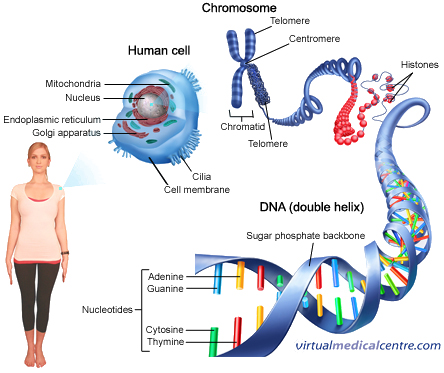
\includegraphics[height = 5cm]{PresentationDNA2.jpg}
}

\frame{\frametitle{What is next-generation sequencing?}

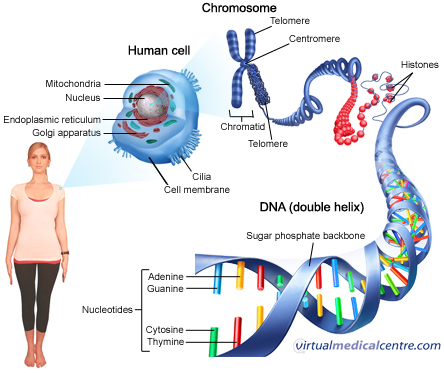
\includegraphics[height = 5cm]{PresentationDNA.jpg}$\hspace*{.3cm}$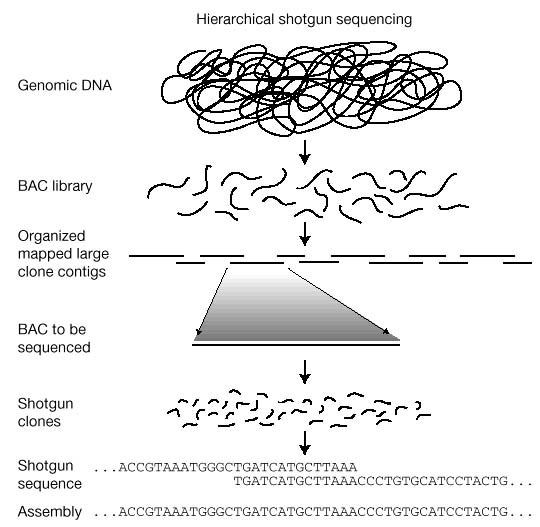
\includegraphics[height = 5cm]{PresentationWhatIsAssembly.jpg}
}

{
\usebackgroundtemplate{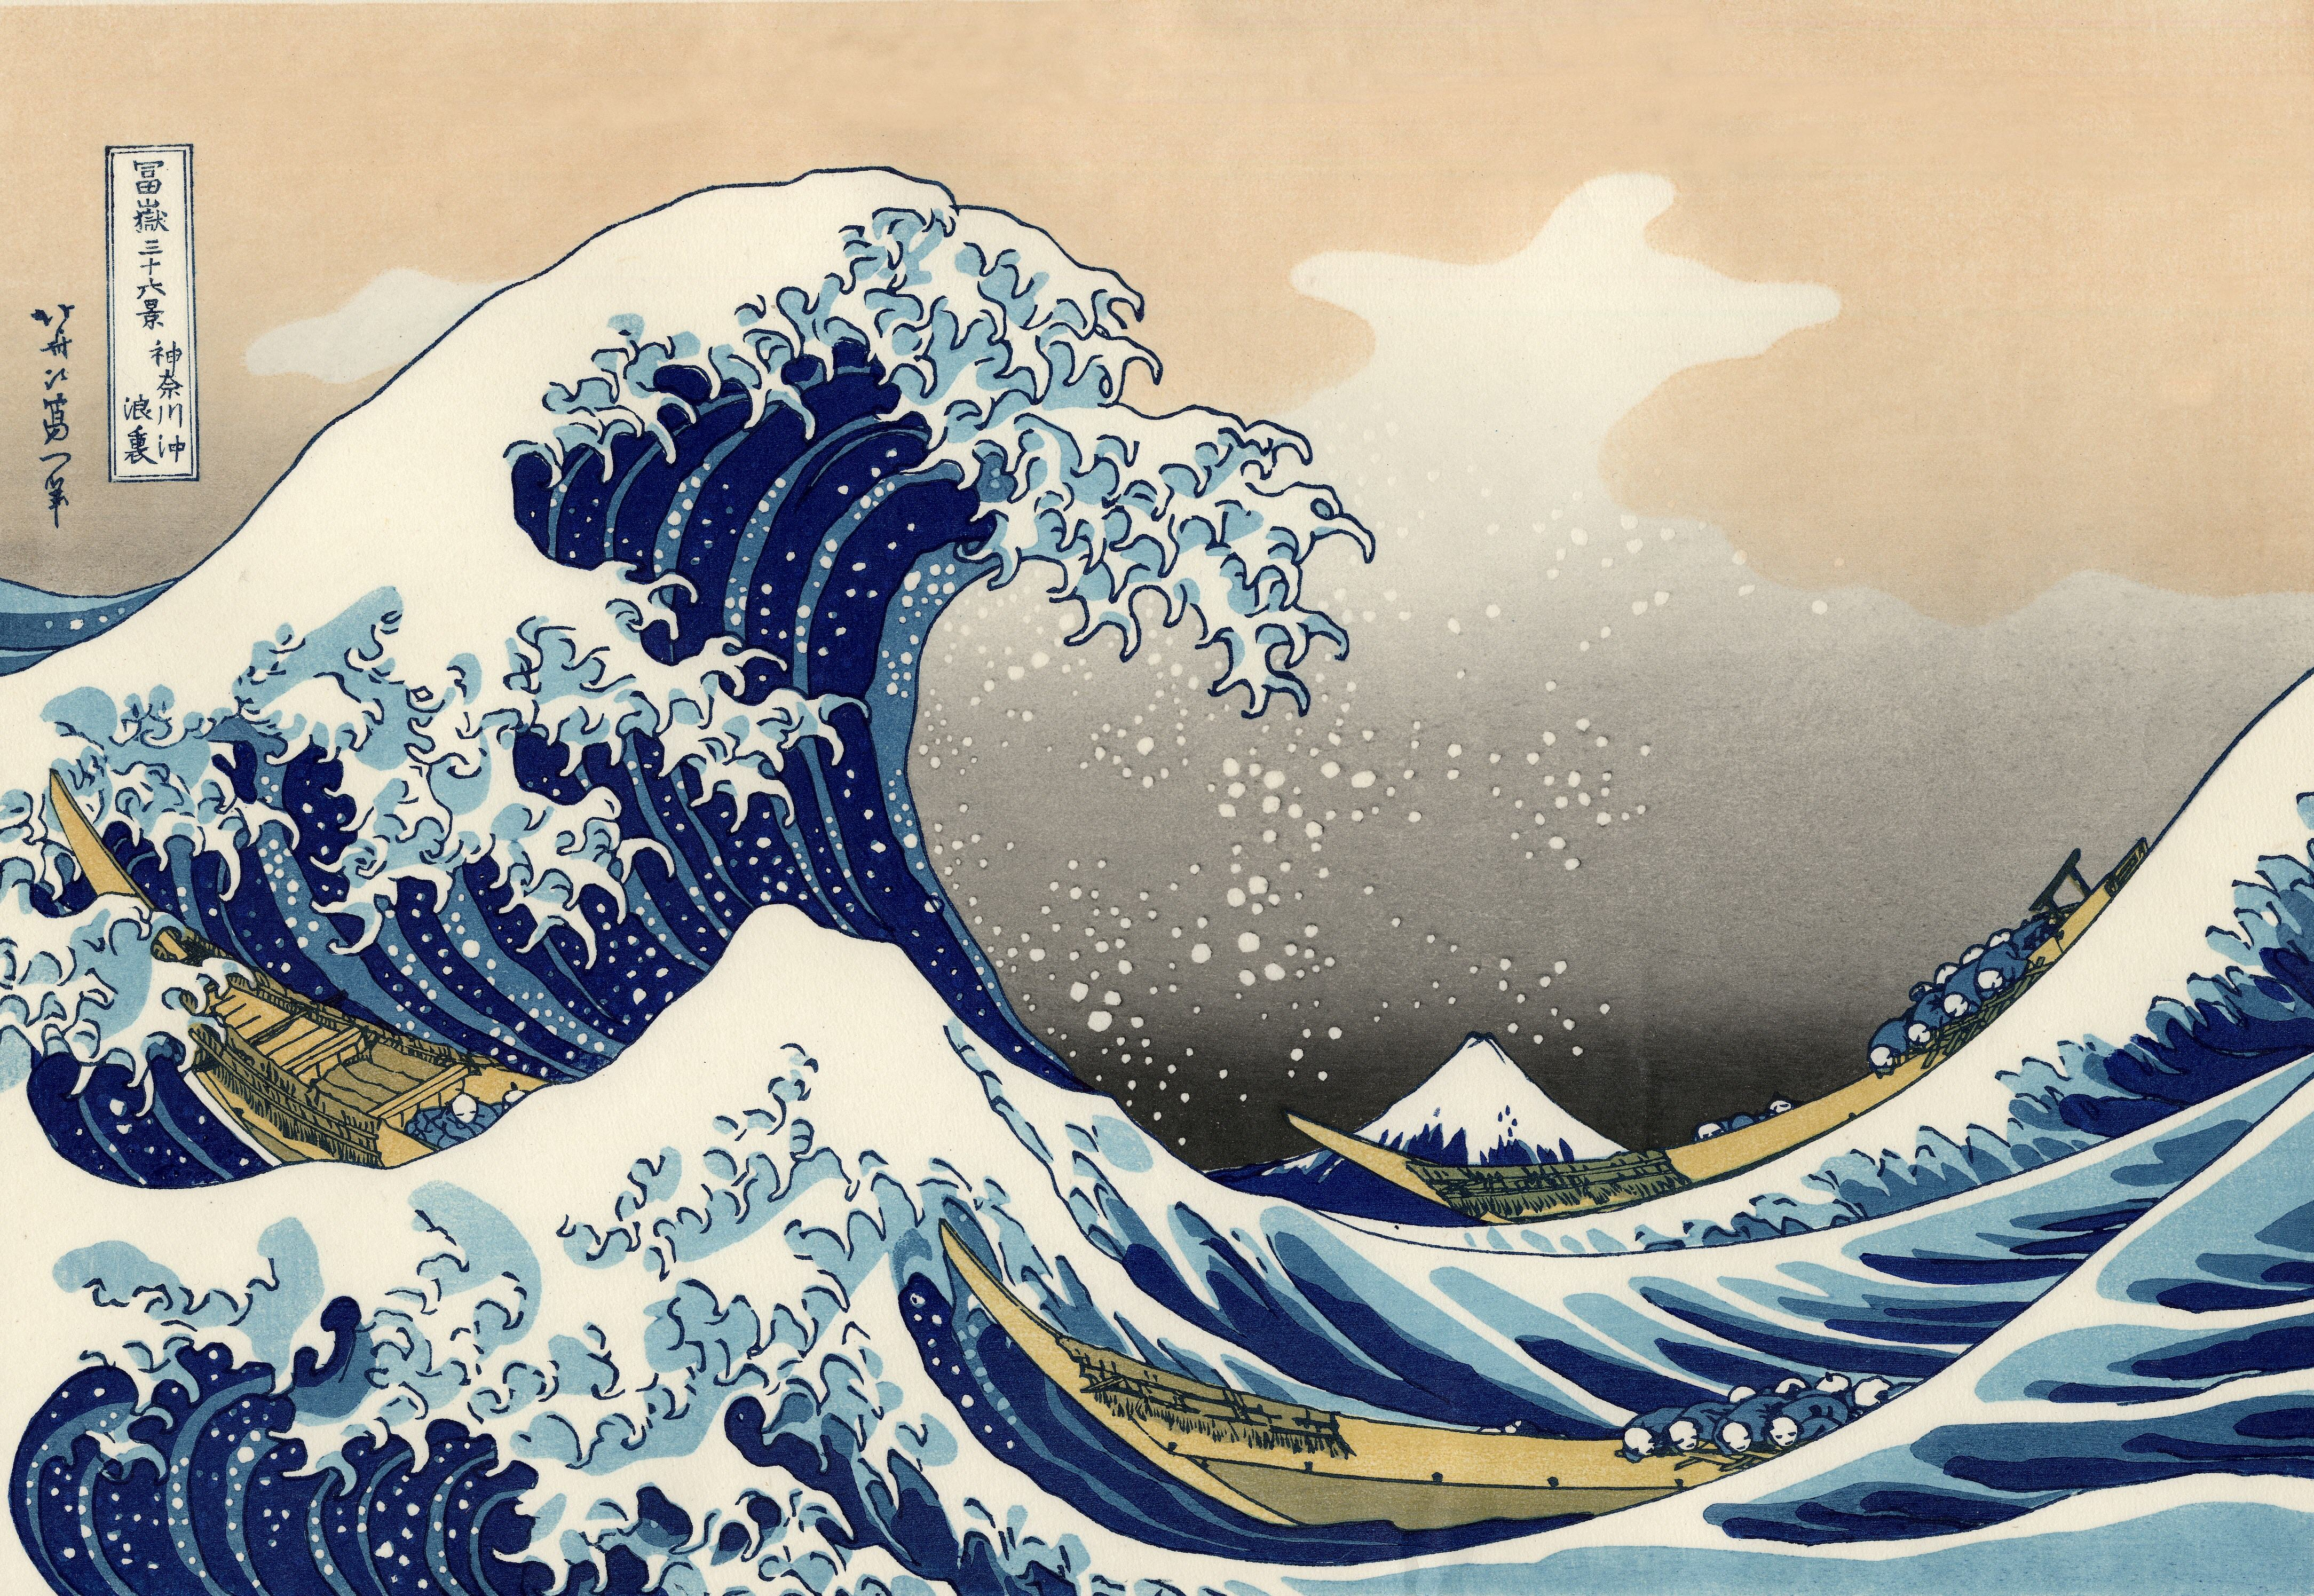
\includegraphics[width=\paperwidth]{PresentationWave.jpg}}

\subsection{Why is it a problem?}
\frame{\frametitle{What is the problem?}

%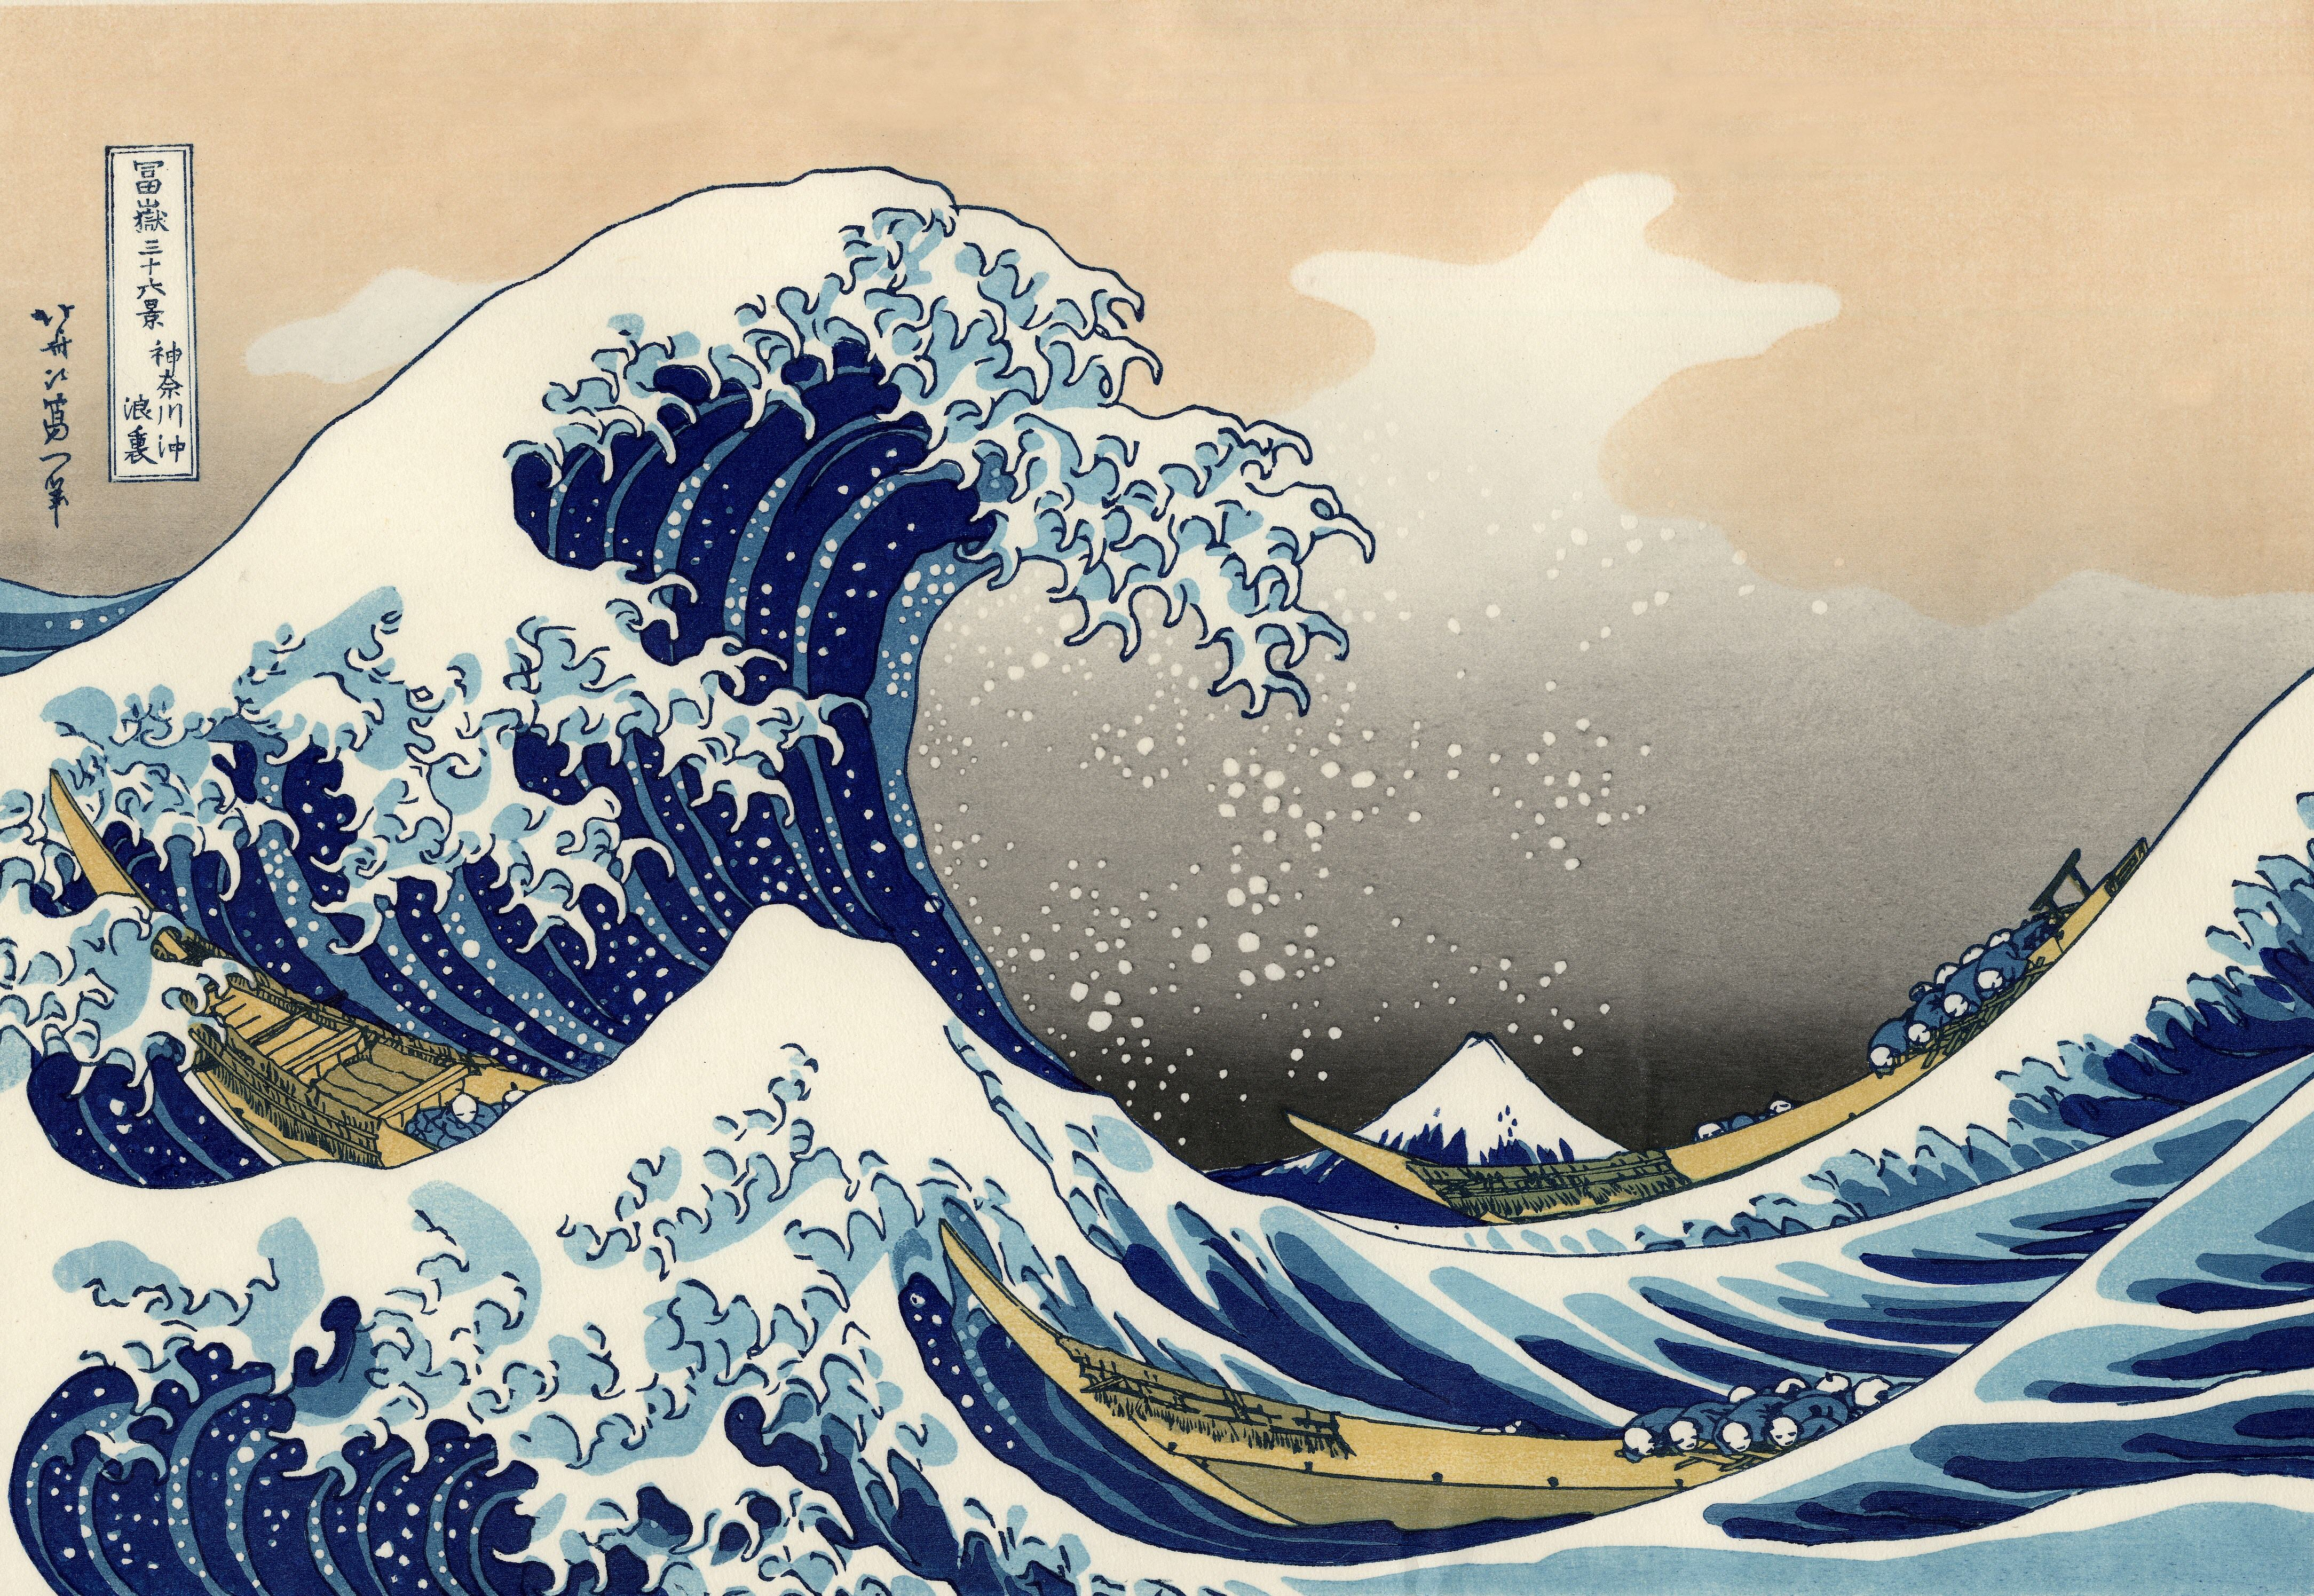
\includegraphics[height = 7cm]{PresentationWave.jpg}

%\framebox{      % just so you can see where the "picture" is
  \begin{picture}(0.1,0.1)
     \put(165,63){\textbf{\huge{A torrent of data}}}
  \end{picture}
%}

%\framebox{      % just so you can see where the "picture" is
  \begin{picture}(0.1,0.1)
     \put(180,62){\textbf{Terabases ($10^{12}$ bp)}}
  \end{picture}
%}

%\framebox{      % just so you can see where the "picture" is
  \begin{picture}(0.1,0.1)
     \put(200,62){\textbf{of sequence}}
  \end{picture}
%}
}
}

{
\usebackgroundtemplate{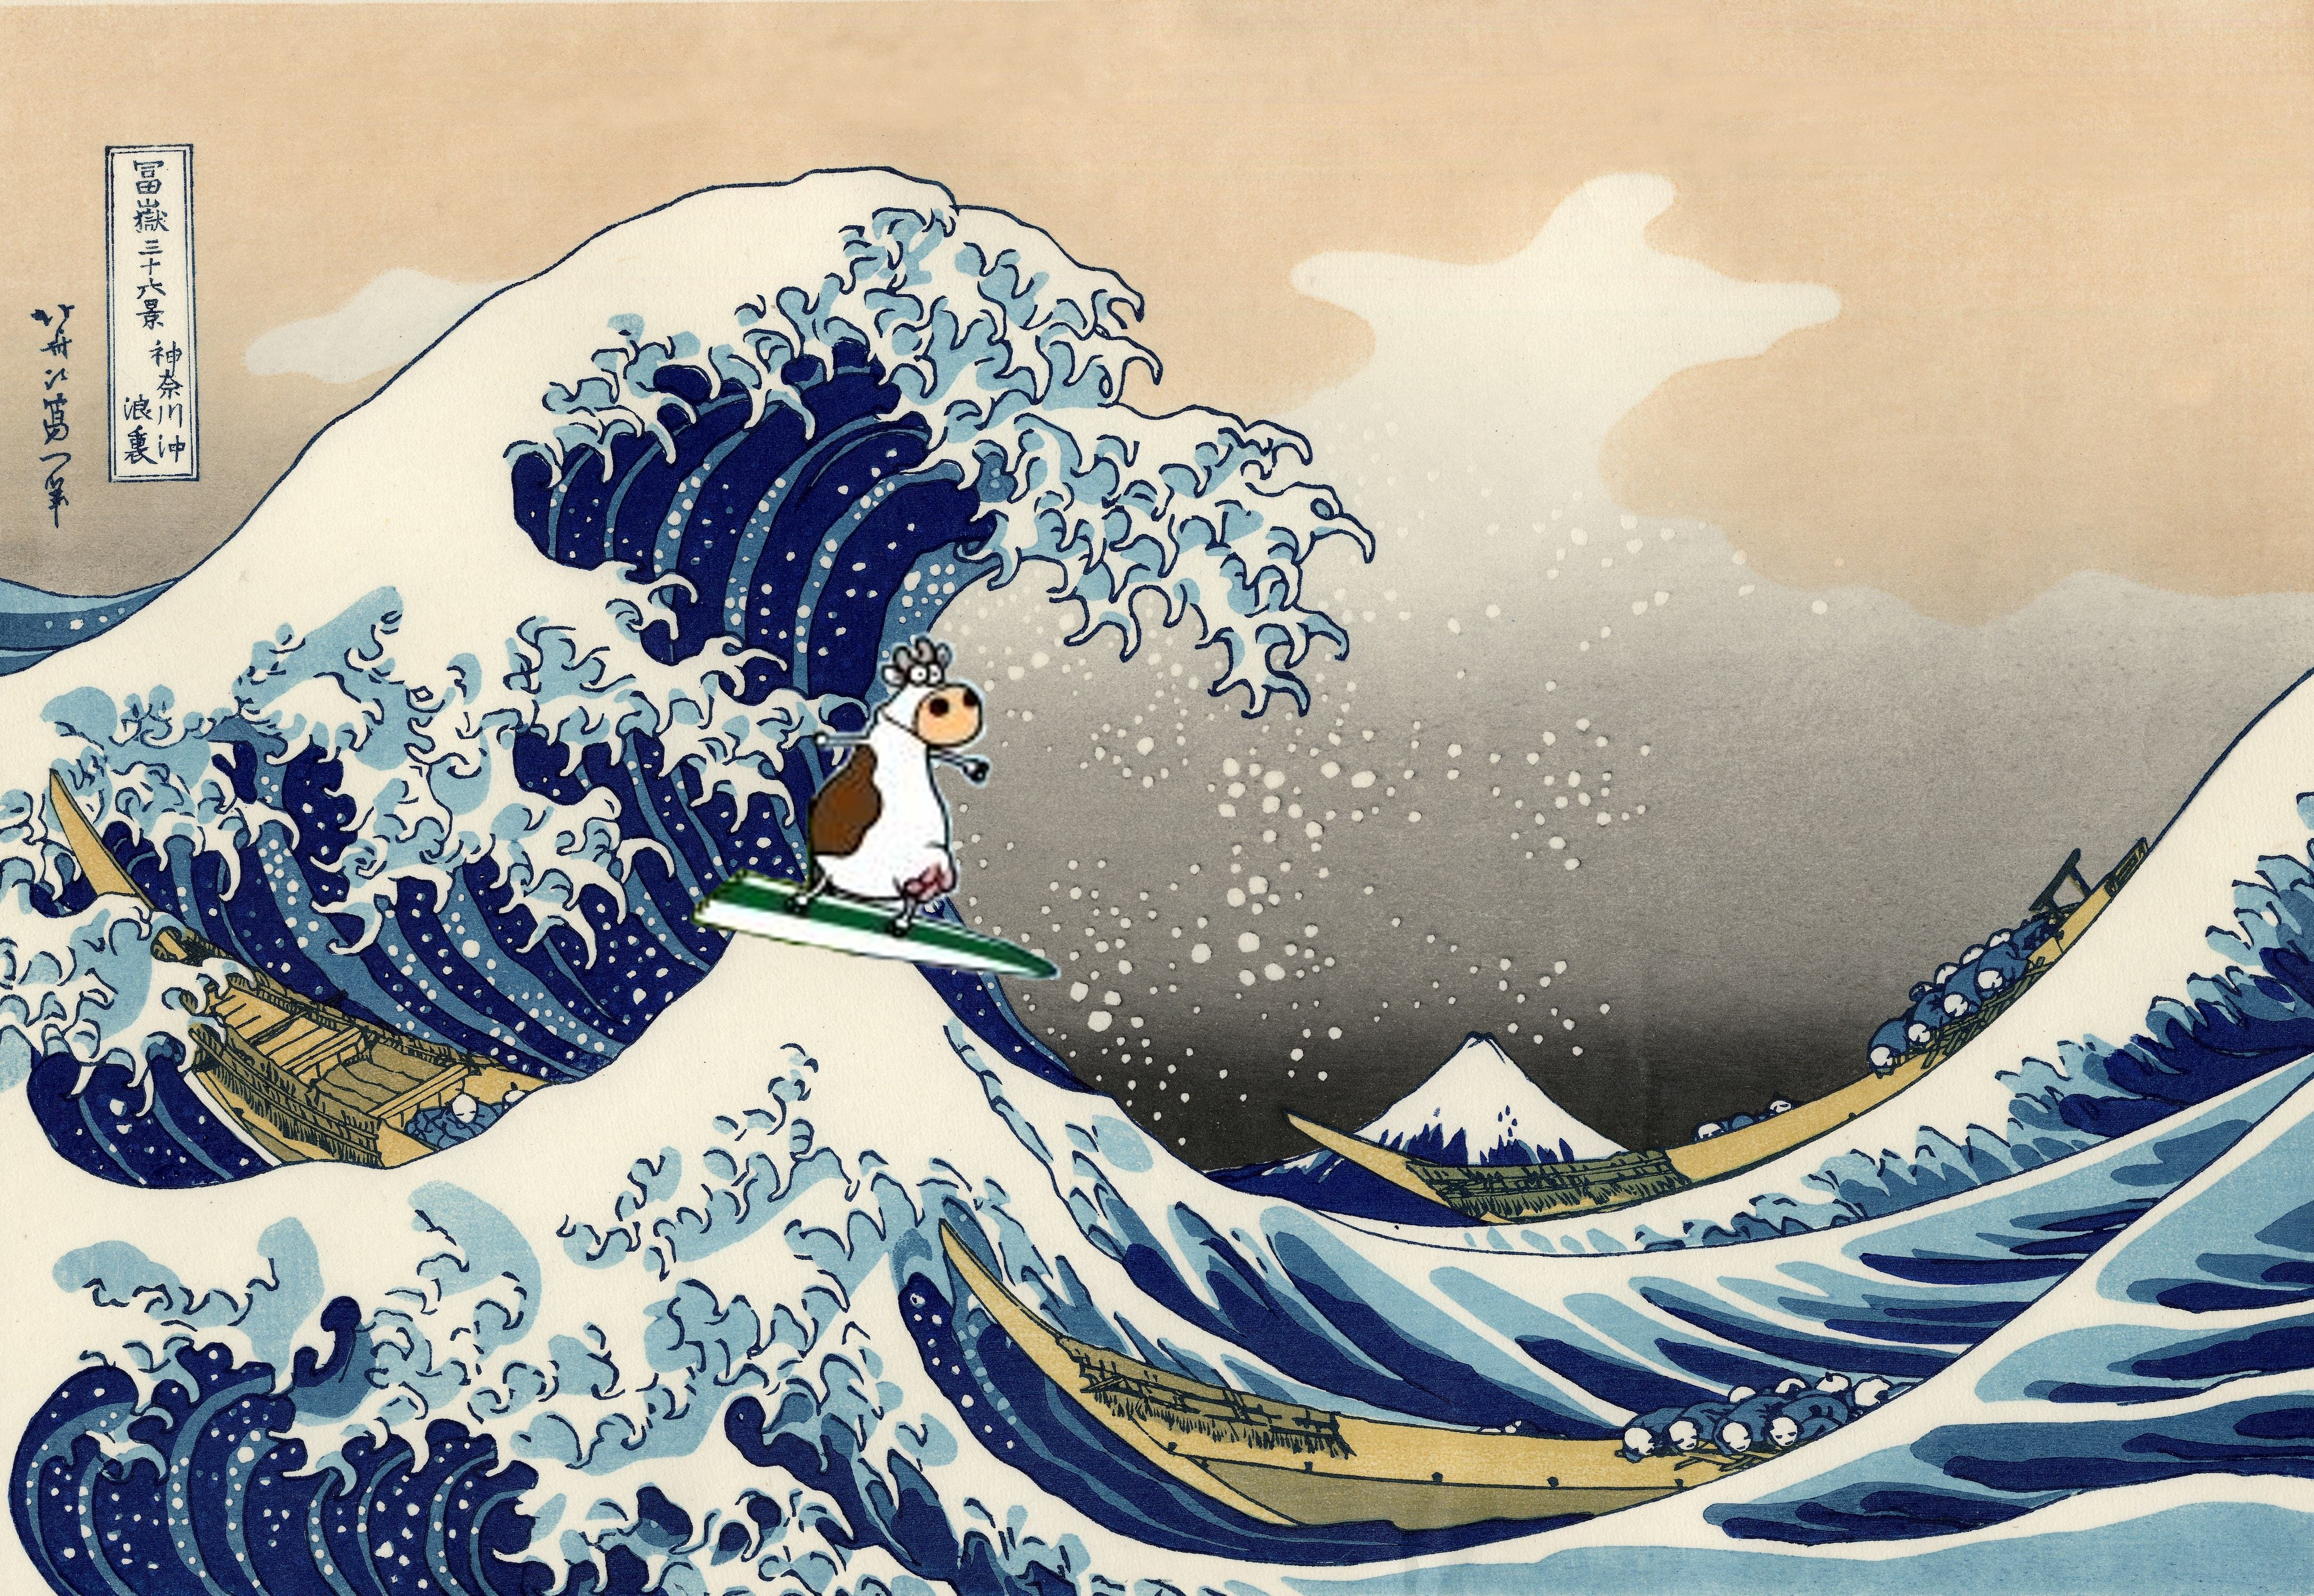
\includegraphics[width=\paperwidth]{PresentationWaveCow.jpg}}

\frame{\frametitle{What is the problem?}

%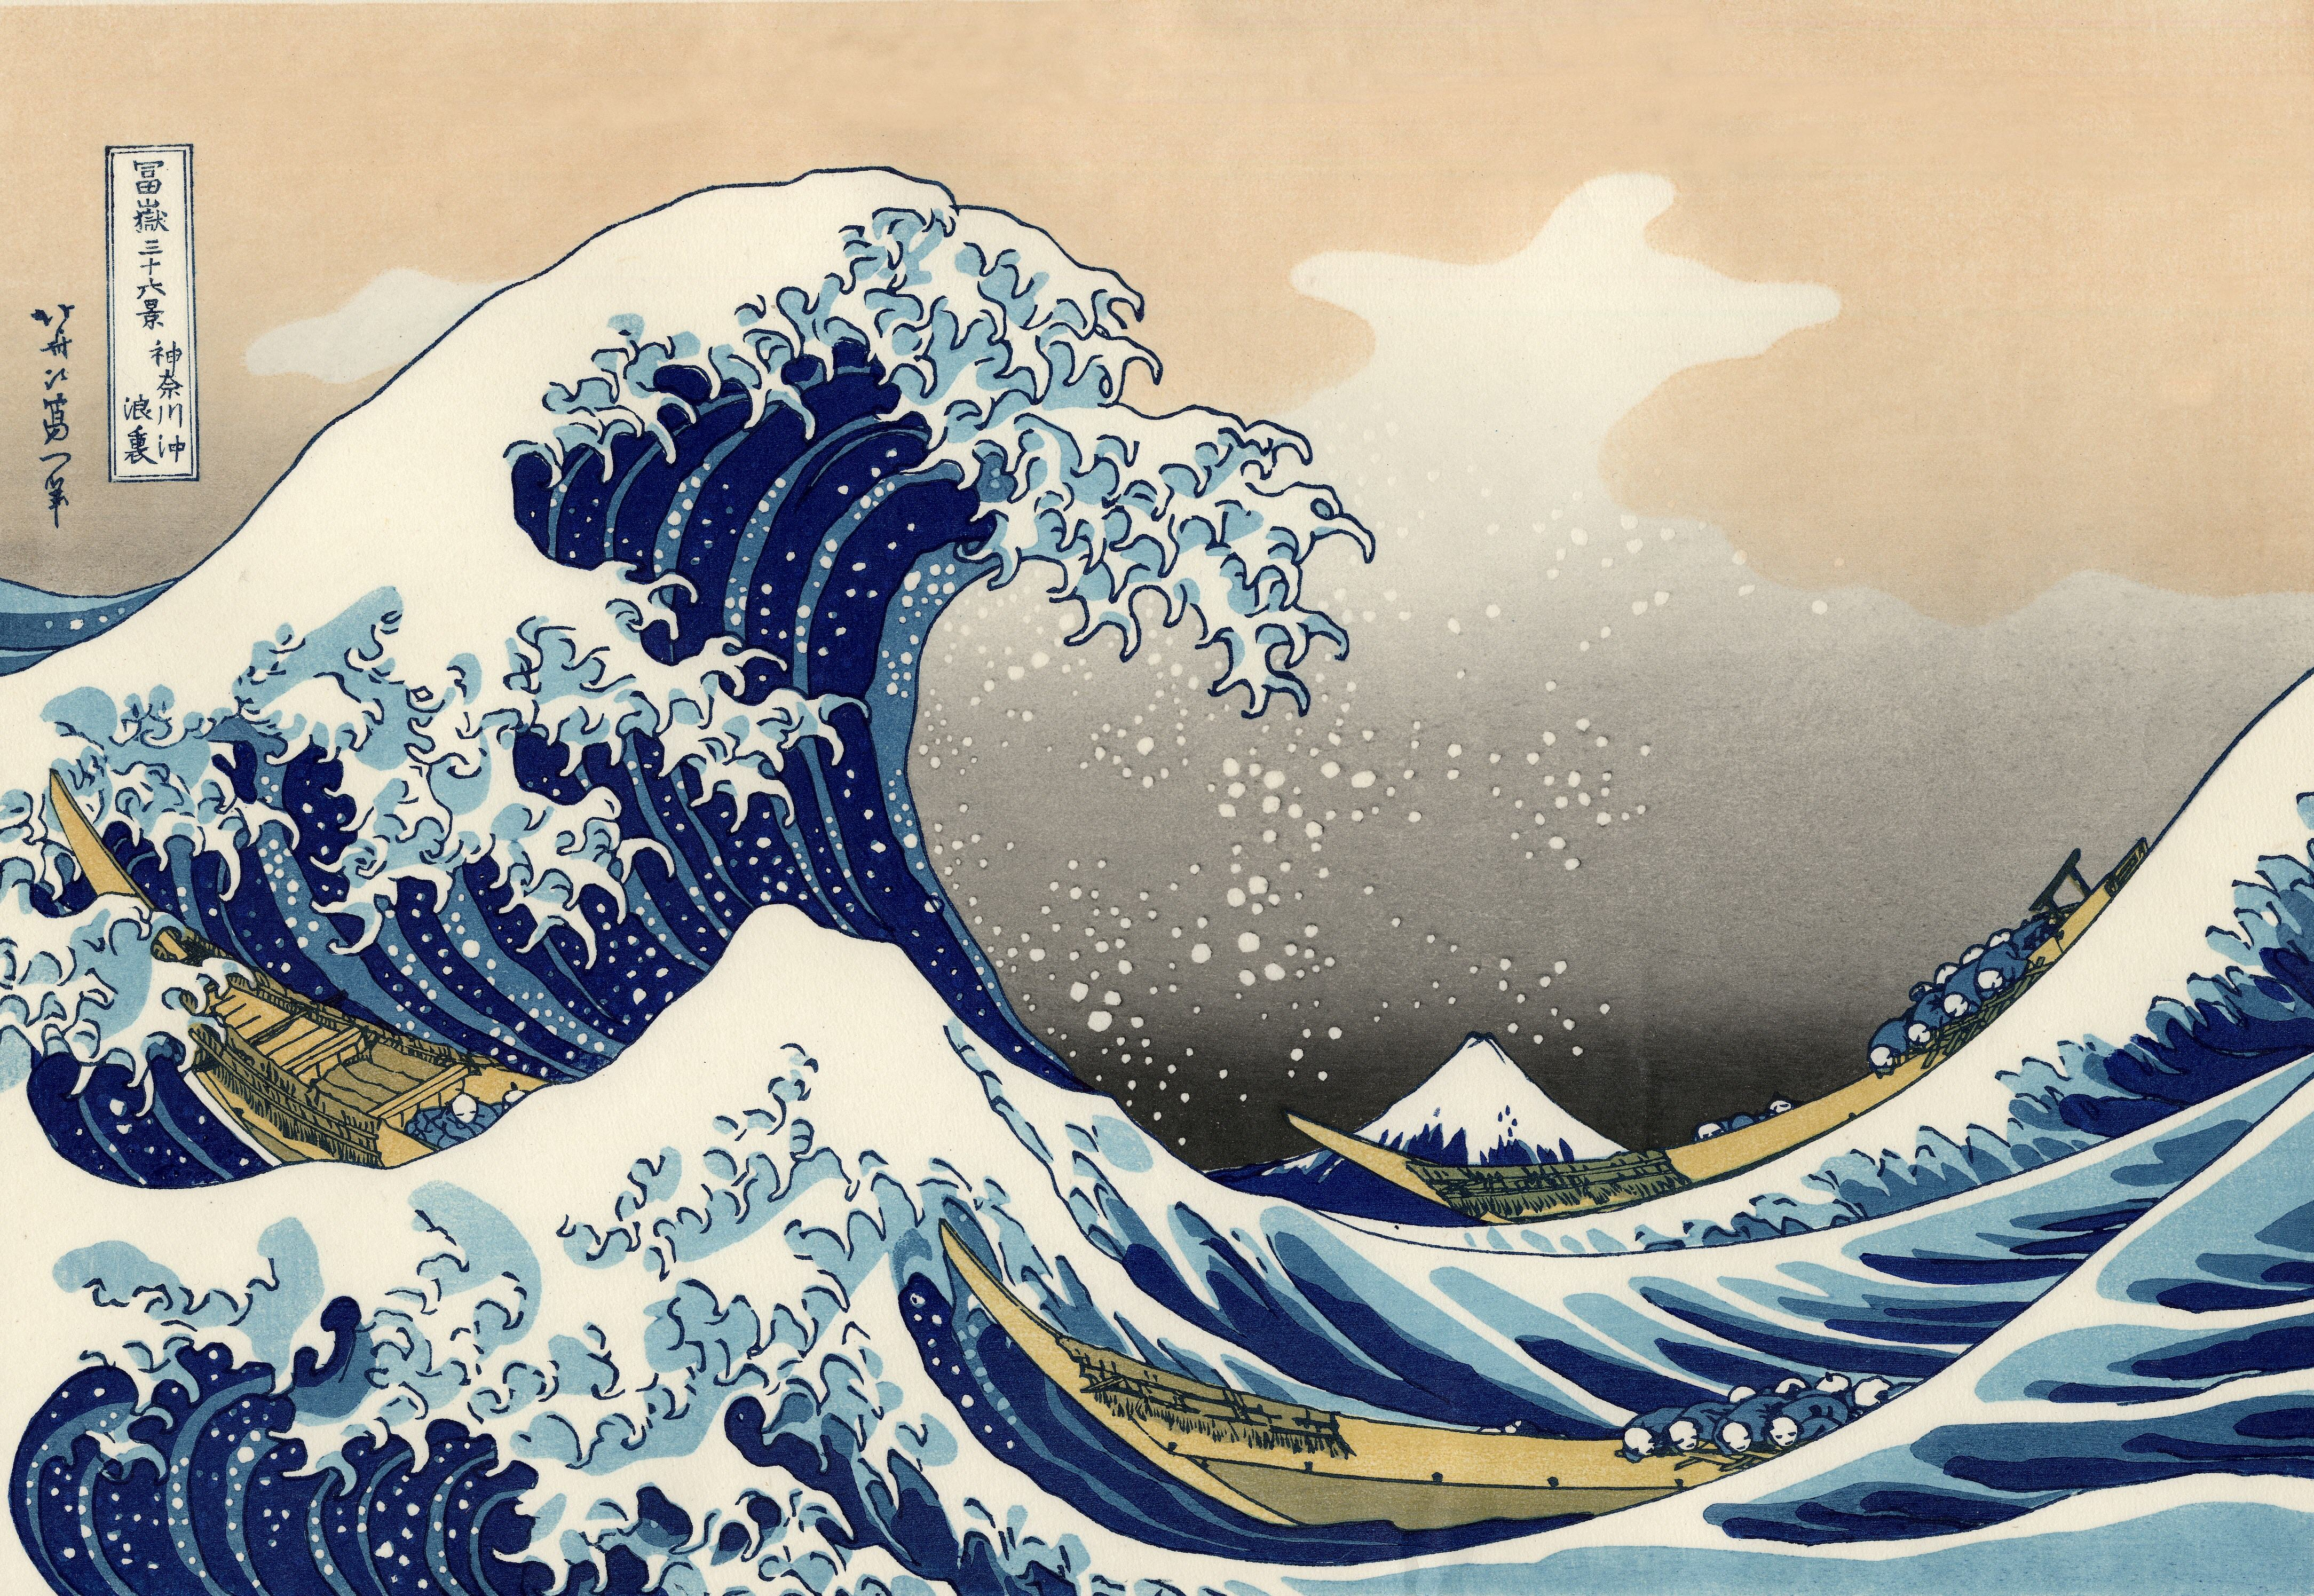
\includegraphics[height = 7cm]{PresentationWave.jpg}

%\framebox{      % just so you can see where the "picture" is
  \begin{picture}(0.1,0.1)
     \put(165,47){\textbf{\huge{A torrent of data}}}
  \end{picture}
%}

%\framebox{      % just so you can see where the "picture" is
  \begin{picture}(0.1,0.1)
     \put(180,46){\textbf{Terabases ($10^{12}$ bp)}}
  \end{picture}
%}

%\framebox{      % just so you can see where the "picture" is
  \begin{picture}(0.1,0.1)
     \put(200,45.5){\textbf{of sequence}}
  \end{picture}
%}

\begin{picture}(0,0)
     \put(195,20){\textbf{\huge{Metagenomes}}}
  \end{picture}

\begin{picture}(0,0)
     \put(195,18){\textbf{like cow rumen}}
  \end{picture}

\begin{picture}(0,0)
     \put(145,18){\textbf{contains many ($\approx10^{3}$) genomes}}
  \end{picture}
}

}

\subsection{Why is it important?}
\frame{\frametitle{Why do we (or the DOE) care?}
\begin{center}
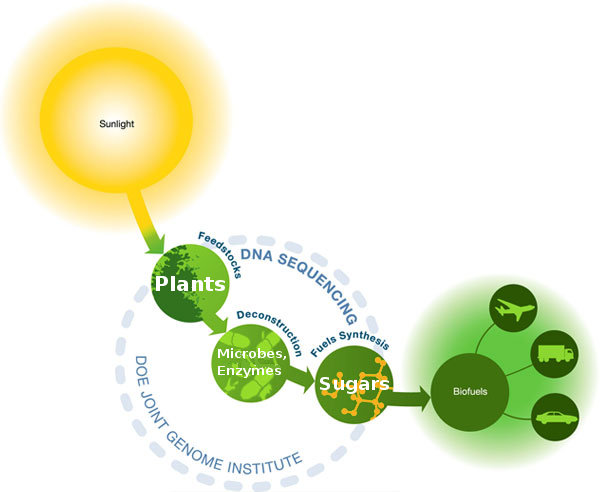
\includegraphics[height = 7cm]{dnaFuel.jpg}\end{center}

}

\frame{\frametitle{Why do we (or the DOE) care?}
\begin{center}
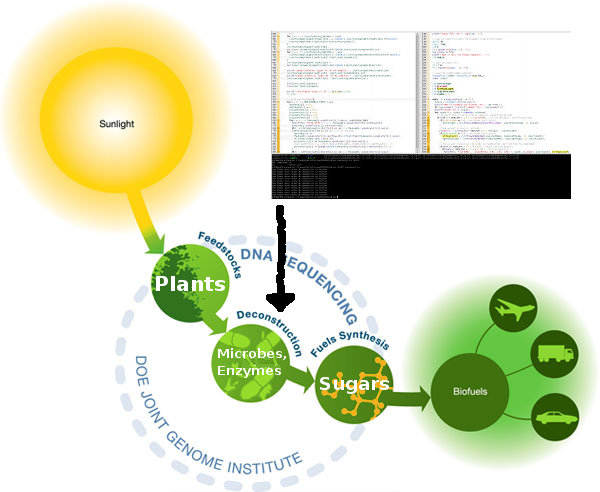
\includegraphics[height = 7cm]{dnaFuel2.jpg}\end{center}

}

\section{Validating Assemblies}
\frame{\frametitle{What is an assembly?}

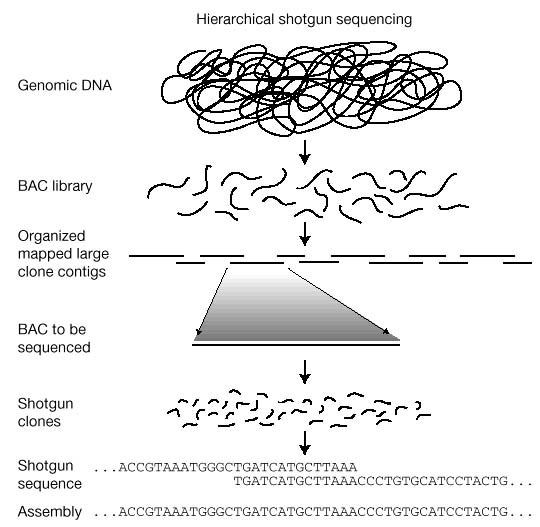
\includegraphics[height = 5cm]{PresentationWhatIsAssembly.jpg}$\hspace*{1cm}$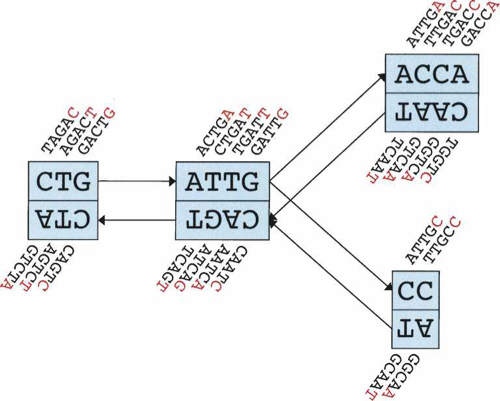
\includegraphics[height = 4cm]{PresentationDeBruijn.png}

}

\subsection{Background}
\frame{\frametitle{What is an assembly?}

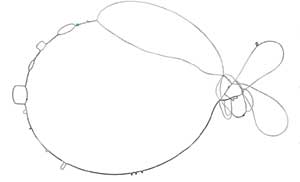
\includegraphics[height = 4cm]{PresentationGraph.jpg}$\hspace*{1cm}$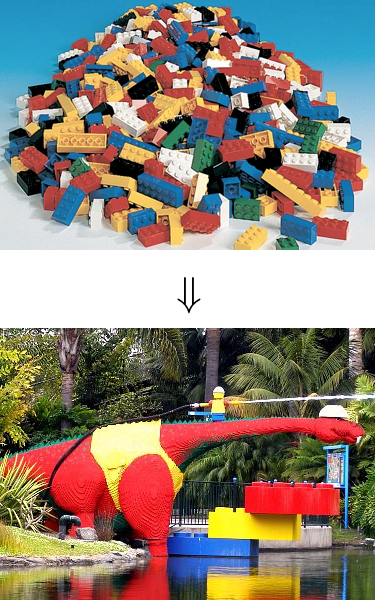
\includegraphics[height = 5cm]{PresentationLego1and2.png}

}

{
\usebackgroundtemplate{
\includegraphics[width=\paperwidth]{DNAp2.jpg}}

\frame{\frametitle{Current methods}

Once we have an assembly from some method we want to know how good it is.

\begin{itemize}
 \item <1->Current Methods
 \begin{enumerate}
  \item Size of pieces (contigs), ie N50 size
  \item Map it onto a known reference
  \item Pathway analysis
 \end{enumerate}
 \item <2->Problems
 \begin{enumerate}
  \item Accuracy irrelevant
  \item Sometimes there is no known reference
  \item Only works on specific pathway (with known reference)
 \end{enumerate}
\end{itemize}
}

\frame{\frametitle{Using Bayes to build likelihoods}

We want to be able to take an assembly and the reads that generated it and find a score, or how likely that assembly is,

\[P\left(\text{Assembly} \left| \text{All the Reads} \right. \right)\]

Which by Bayes rule is proportional to

\[P\left(\text{All the Reads} \left| \text{Assembly} \right. \right)\]

This will be our likelihood function.

}




\subsection{Our likelihood function}
\frame{\frametitle{Read properties}

\begin{figure}[!htpb]
\begin{center}
\textbf{Mated Read $R_{k}$ Properties}
\[\text{Read $R_{k}$: }\overbrace{\underbrace{\text{{\color{red} A}{\color{blue} T}{\color{MyDarkGreen} C}{\color{orange} G}{\color{MyDarkGreen} C}{\color{MyDarkGreen} C}{\color{blue} T}{\color{orange} G}{\color{red} A}{\color{blue} T}{\color{blue} T}{\color{MyDarkGreen} C}}}_{\text{length: } L\left(R_{k}^{(1)}\right) \sim \Theta_{L_{k}}}}^{\text{Mate Pair \#1: } R_{k}^{(1)}}
\overbrace{\underbrace{\text{{\color{gray} ATTCGAGTCGA}}}_{\text{length: } I_{k} \sim \Theta_{I_{k}}}}^{\text{Insert Area}}
\overbrace{\underbrace{\text{{\color{blue} T}{\color{MyDarkGreen} C}{\color{red} A}{\color{blue} T}{\color{MyDarkGreen} C}{\color{blue} T}{\color{MyDarkGreen} C}{\color{orange} G}{\color{red} A}{\color{blue} T}{\color{orange} G}{\color{MyDarkGreen} C}{\color{red} A}}}_{\text{length: } L\left(R_{k}^{(2)}\right) \sim \Theta_{L_{k}}}}^{\text{Mate Pair \#2: } R_{k}^{(2)}}\]
\end{center}
\label{readProp}
\end{figure}

\begin{figure}[!htpb]
\textbf{Orientation $\omega_{k}$ of mated read $R_{k}$}
\begin{center}
$\overbrace{\hspace*{9cm}}^{\omega_{k} = +1}$
\begin{tabular}{ccc}
$\xrightarrow{\hspace*{3cm}}$ & Inward & $\xleftarrow{\hspace*{3.3cm}}$ \\
{\color{red} A}{\color{blue} T}{\color{MyDarkGreen} C}{\color{orange} G}{\color{MyDarkGreen} C}{\color{MyDarkGreen} C}{\color{blue} T}{\color{orange} G}{\color{red} A}{\color{blue} T}{\color{blue} T}{\color{MyDarkGreen} C} & $\hdots\hdots$ & {\color{blue} T}{\color{MyDarkGreen} C}{\color{red} A}{\color{blue} T}{\color{MyDarkGreen} C}{\color{blue} T}{\color{MyDarkGreen} C}{\color{orange} G}{\color{red} A}{\color{blue} T}{\color{orange} G}{\color{MyDarkGreen} C}{\color{red} A} \\
$\xleftarrow{\hspace*{3cm}}$ & Outward & $\xrightarrow{\hspace*{3.3cm}}$
\end{tabular}
$\underbrace{\hspace*{9cm}}_{\omega_{k} = -1}$
\end{center}
\label{readOr}
\end{figure}

}

\frame{\frametitle{Components of the likelihood function}

The Likelihood needs to take at least the following into account:
\begin{itemize}
 \item Read \textbf{sequences} need to agree with assembly.
 \item \textbf{Insert lengths} must be consistent.
 \item \textbf{Orientation} of mated reads needs to be consistent.
 \item \textbf{Number of reads mapping} onto the assembly.
 \item \textbf{Coverage} normally distributed.
 \item \textbf{$k$-\textit{mer} frequency} must be consistent. (within a contig)
\end{itemize}
}

\frame{\frametitle{ALE placement score}

\begin{center}
\begin{tabular}{cc}
    Seed $S$ & $\cdots\overset{51}{\text{{\color{MyDarkGreen}C}}}\text{{\color{orange} G}{\color{red} A}}\text{{\color{red} A}}\overset{55}{\text{{\color{blue} T}}} \text{{\color{MyDarkGreen} C}{\color{orange} G}{\color{MyDarkGreen} C}{\color{MyDarkGreen} C}}\overset{60}{\text{{\color{blue} T}}}\text{{\color{orange} G}{\color{red} A}{\color{blue} T}{\color{blue} T}}\overset{65}{\text{{\color{MyDarkGreen} C}}}\text{{\color{red} A}{\color{blue} T}{\color{blue} T}{\color{MyDarkGreen} C}}\overset{70}{\text{{\color{orange} G}}}$\\
    read $r_{k}$ & \text{{\color{white}$\cdots$GCA}}$\underrightarrow{\text{{\color{red} A}{\color{blue} T}{\color{MyDarkGreen} C}{\color{orange} G}{\color{MyDarkGreen} C}{\color{MyDarkGreen} C}{\color{blue} T}{\color{orange} G}{\color{red} A}{\color{blue} T}{\color{blue} T}{\color{MyDarkGreen} C}}}$\text{{\color{white} A}{\color{white} T}{\color{white} T}{\color{white} C}{\color{white} G}}
\end{tabular}
\end{center}

\[P_{\text{matches}}\left(r_{i}|S\right)(j) = \left\{\begin{tabular}{cc} $Q_{j}$ & if $r_{k}(j) = S(j+\Omega)$ \\ $\frac{1-Q_{j}}{4}$ & if $r_{k}(j) \neq S(j+\Omega)$ \end{tabular}\right.\]

\[P_{\text{placement}}\left(r_{i}|S\right) = P_{\text{matches}}\left(r_{i}|S\right)P_{\text{orientation}}\left(r_{i}|S\right)\]

}

\frame{\frametitle{ALE insert score}
Total ALE score needs to take insert size into account

\footnotesize
\begin{tabular}{cc} \\

$S$ & \text{$\cdots\overset{51}{\text{{\color{MyDarkGreen}C}}}${\color{orange} G}{\color{red} A}}$\text{{\color{red} A}$\overset{55}{\text{{\color{blue} T}}}${\color{MyDarkGreen} C}{\color{orange} G}{\color{MyDarkGreen} C}{\color{MyDarkGreen} C}$\overset{60}{\text{{\color{blue} T}}}${\color{orange} G}{\color{red} A}{\color{blue} T}{\color{blue} T}$\overset{65}{\text{{\color{MyDarkGreen} C}}}$}$\text{{\color{red} A}{\color{blue} T}{\color{blue} T}{\color{MyDarkGreen} C}$\overset{70}{\text{{\color{orange} G}}}${\color{red} A}{\color{orange} G}{\color{blue} T}{\color{MyDarkGreen} C}$\overset{75}{\text{{\color{orange} G}}}${\color{red} A}}$\text{{\color{blue} T}{\color{MyDarkGreen} C}{\color{red} A}$\overset{80}{\text{{\color{blue} T}}}${\color{MyDarkGreen} C}{\color{blue} T}{\color{MyDarkGreen} C}{\color{orange} G}$\overset{85}{\text{{\color{red} A}}}${\color{blue} T}{\color{orange} G}$\overset{88}{\text{{\color{MyDarkGreen} C}}}$}$\text{N} \\

$r_{k}$ & \text{{\color{white}$\cdots$GCA}}$\underrightarrow{\text{{\color{red} A}{\color{blue} T}{\color{MyDarkGreen} C}{\color{orange} G}{\color{MyDarkGreen} C}{\color{MyDarkGreen} C}{\color{blue} T}{\color{orange} G}{\color{red} A}{\color{blue} T}{\color{blue} T}{\color{MyDarkGreen} C}}}\underset{\text{Implied Insert}}{\underleftrightarrow{\text{{\color{white} A}{\color{white} T}{\color{white} T}{\color{white} C}{\color{white} G}{\color{white} A}{\color{white} G}{\color{white} T}{\color{white} C}{\color{white} G}{\color{white} A}}}}\underleftarrow{\text{{\color{blue} T}{\color{MyDarkGreen} C}{\color{red} A}{\color{blue} T}{\color{MyDarkGreen} C}{\color{blue} T}{\color{MyDarkGreen} C}{\color{orange} G}{\color{red} A}{\color{blue} T}{\color{orange} G}{\color{MyDarkGreen} C}{\color{red} A}}}$
\end{tabular}
\normalsize

\ \\

\[P_{\text{insert}}\left(r_{i}|S\right) = {\rm Normal}\left(L_{i};\mu,\sigma^{2}\right)\]
}



\frame{\frametitle{ALE depth score}
We expect the coverage of the reads when mapped back onto the seeds to be Poisson distributed (Lander 1988)

\[P_{\text{depth}}\left(d_{j}|S,X_{i}\right) = {\rm Poisson}\left(d_{j};Y_{i}\right)\]
\[Y_{i} \sim {\rm Gamma}(\max(10,\mu_{\text{depth}(X_{i})}), 1)\]
\[P_{\text{depth}}\left(d_{j}|S,X_{i}\right) = {\rm NegBinom}(d_{j}; \max(10, \mu_{\text{depth}(X_{i})}), 1/2)\]

GC correction
\begin{itemize}
 \item The sequencing technology introduces a ``GC bias''
 \item Those bases are overrepresented in the data
 \item We compute 100 different Poisson distributions based on the \% of GC in each read
\end{itemize}
}

\frame{\frametitle{ALE depth score: GC bias}
\begin{center}
 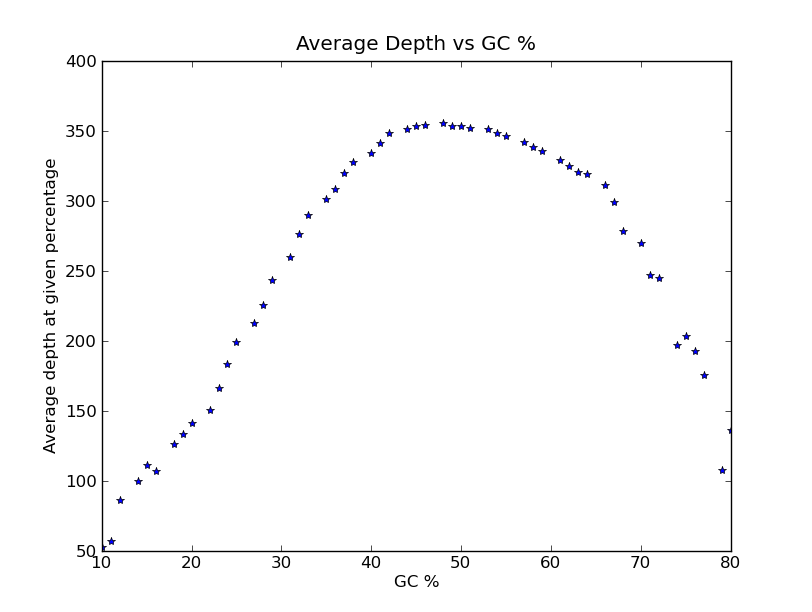
\includegraphics[height = 7cm]{figures/ALE/avgDepthVsGC.png}
\end{center}
}

\frame{\frametitle{ALE kmer score}
What are $k$-mers?
\begin{itemize}
 \item Contiguous subsequences of length $k$
 \item The frequency a $k$-mer appears (for $k \geq 4$) is relatively distinct between species
 \item We can use this information to distinguish individual species from a metagenome
\end{itemize}
\[f_{i} = \frac{n_{i}}{\sum_{j\in K}n_{j}}\]
\[ P_{\text{kmer}}(S) = \prod_{i\in K} f_{i}^{n_{i}}\]
}

\frame{\frametitle{Normalization and total scores}
The total ALE score

\[P(S|R) = \frac{P(R|S)P(S)}{Z}\]

\[P(R|S)=P_{\text{placement}}(R|S)P_{\text{insert}}(R|S)P_{\text{depth}}(R|S)\]

\[P(S) = P_{\text{kmer}}(S)\]

Comparing two assemblies

\[A_{1} - A_{2} = \log\left(\frac{P\left(R|S_{1}\right)P\left(S_{1}\right)}{P\left(R|S_{2}\right)P\left(S_{2}\right)}\right)\]
}

}

\subsection{Results}

\frame{\frametitle{Likelihood with permutation from a known assembly}
\begin{center}
 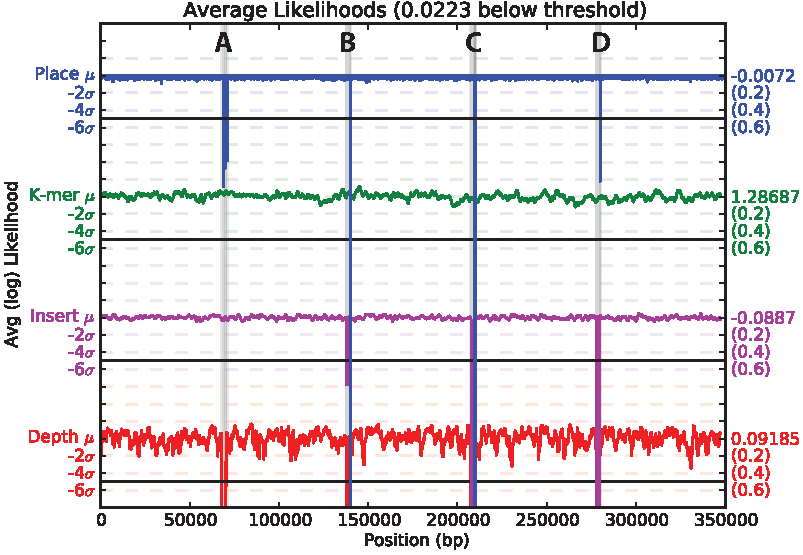
\includegraphics[height = 7cm]{figures/ALE/fig_2_top.pdf}
\end{center}
}

\frame{\frametitle{Likelihood with permutation from a known assembly}
\begin{center}
 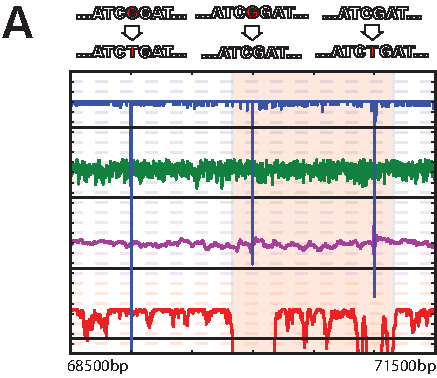
\includegraphics[height = 7cm]{figures/ALE/fig2_bot_p1.pdf}
\end{center}
}

\frame{\frametitle{Likelihood with permutation from a known assembly}
\begin{center}
 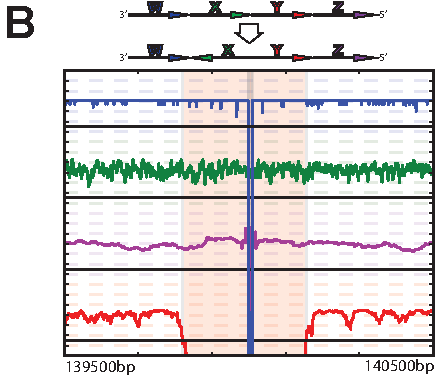
\includegraphics[height = 7cm]{figures/ALE/fig2_bot_p2.pdf}
\end{center}
}

\frame{\frametitle{Likelihood with permutation from a known assembly}
\begin{center}
 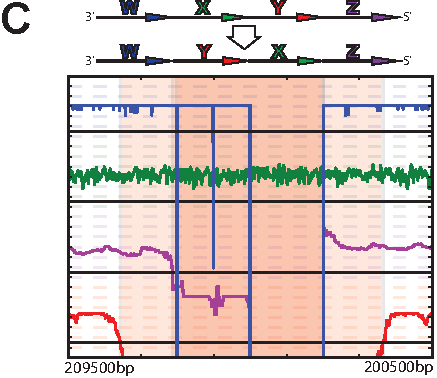
\includegraphics[height = 7cm]{figures/ALE/fig2_bot_p3.pdf}
\end{center}
}

\frame{\frametitle{Likelihood with permutation from a known assembly}
\begin{center}
 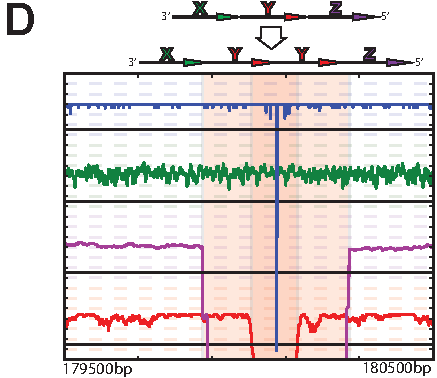
\includegraphics[height = 7cm]{figures/ALE/fig2_bot_p4.pdf}
\end{center}
}

\frame{\frametitle{Likelihood vs \# permutations from a known assembly}
\begin{center}
 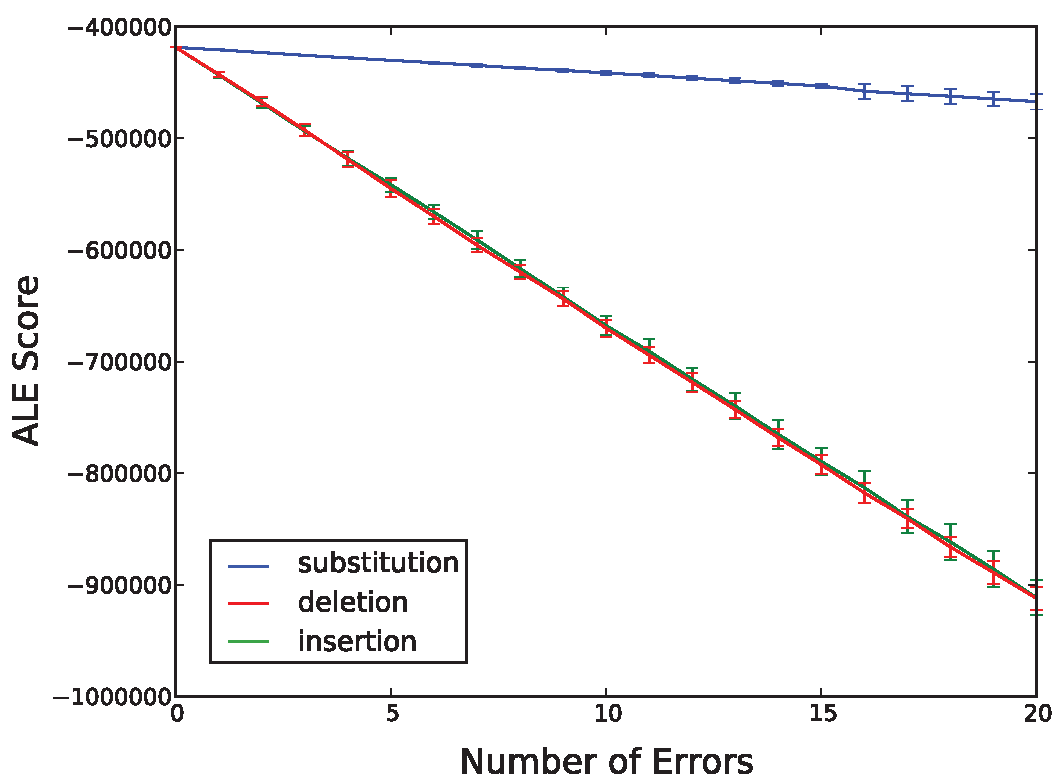
\includegraphics[height = 7cm]{figures/ALE/Clark_Fig3b.pdf}
\end{center}
}

\frame{\frametitle{Detecting chimeric assemblies in a synthetic metagenome}
\begin{center}
 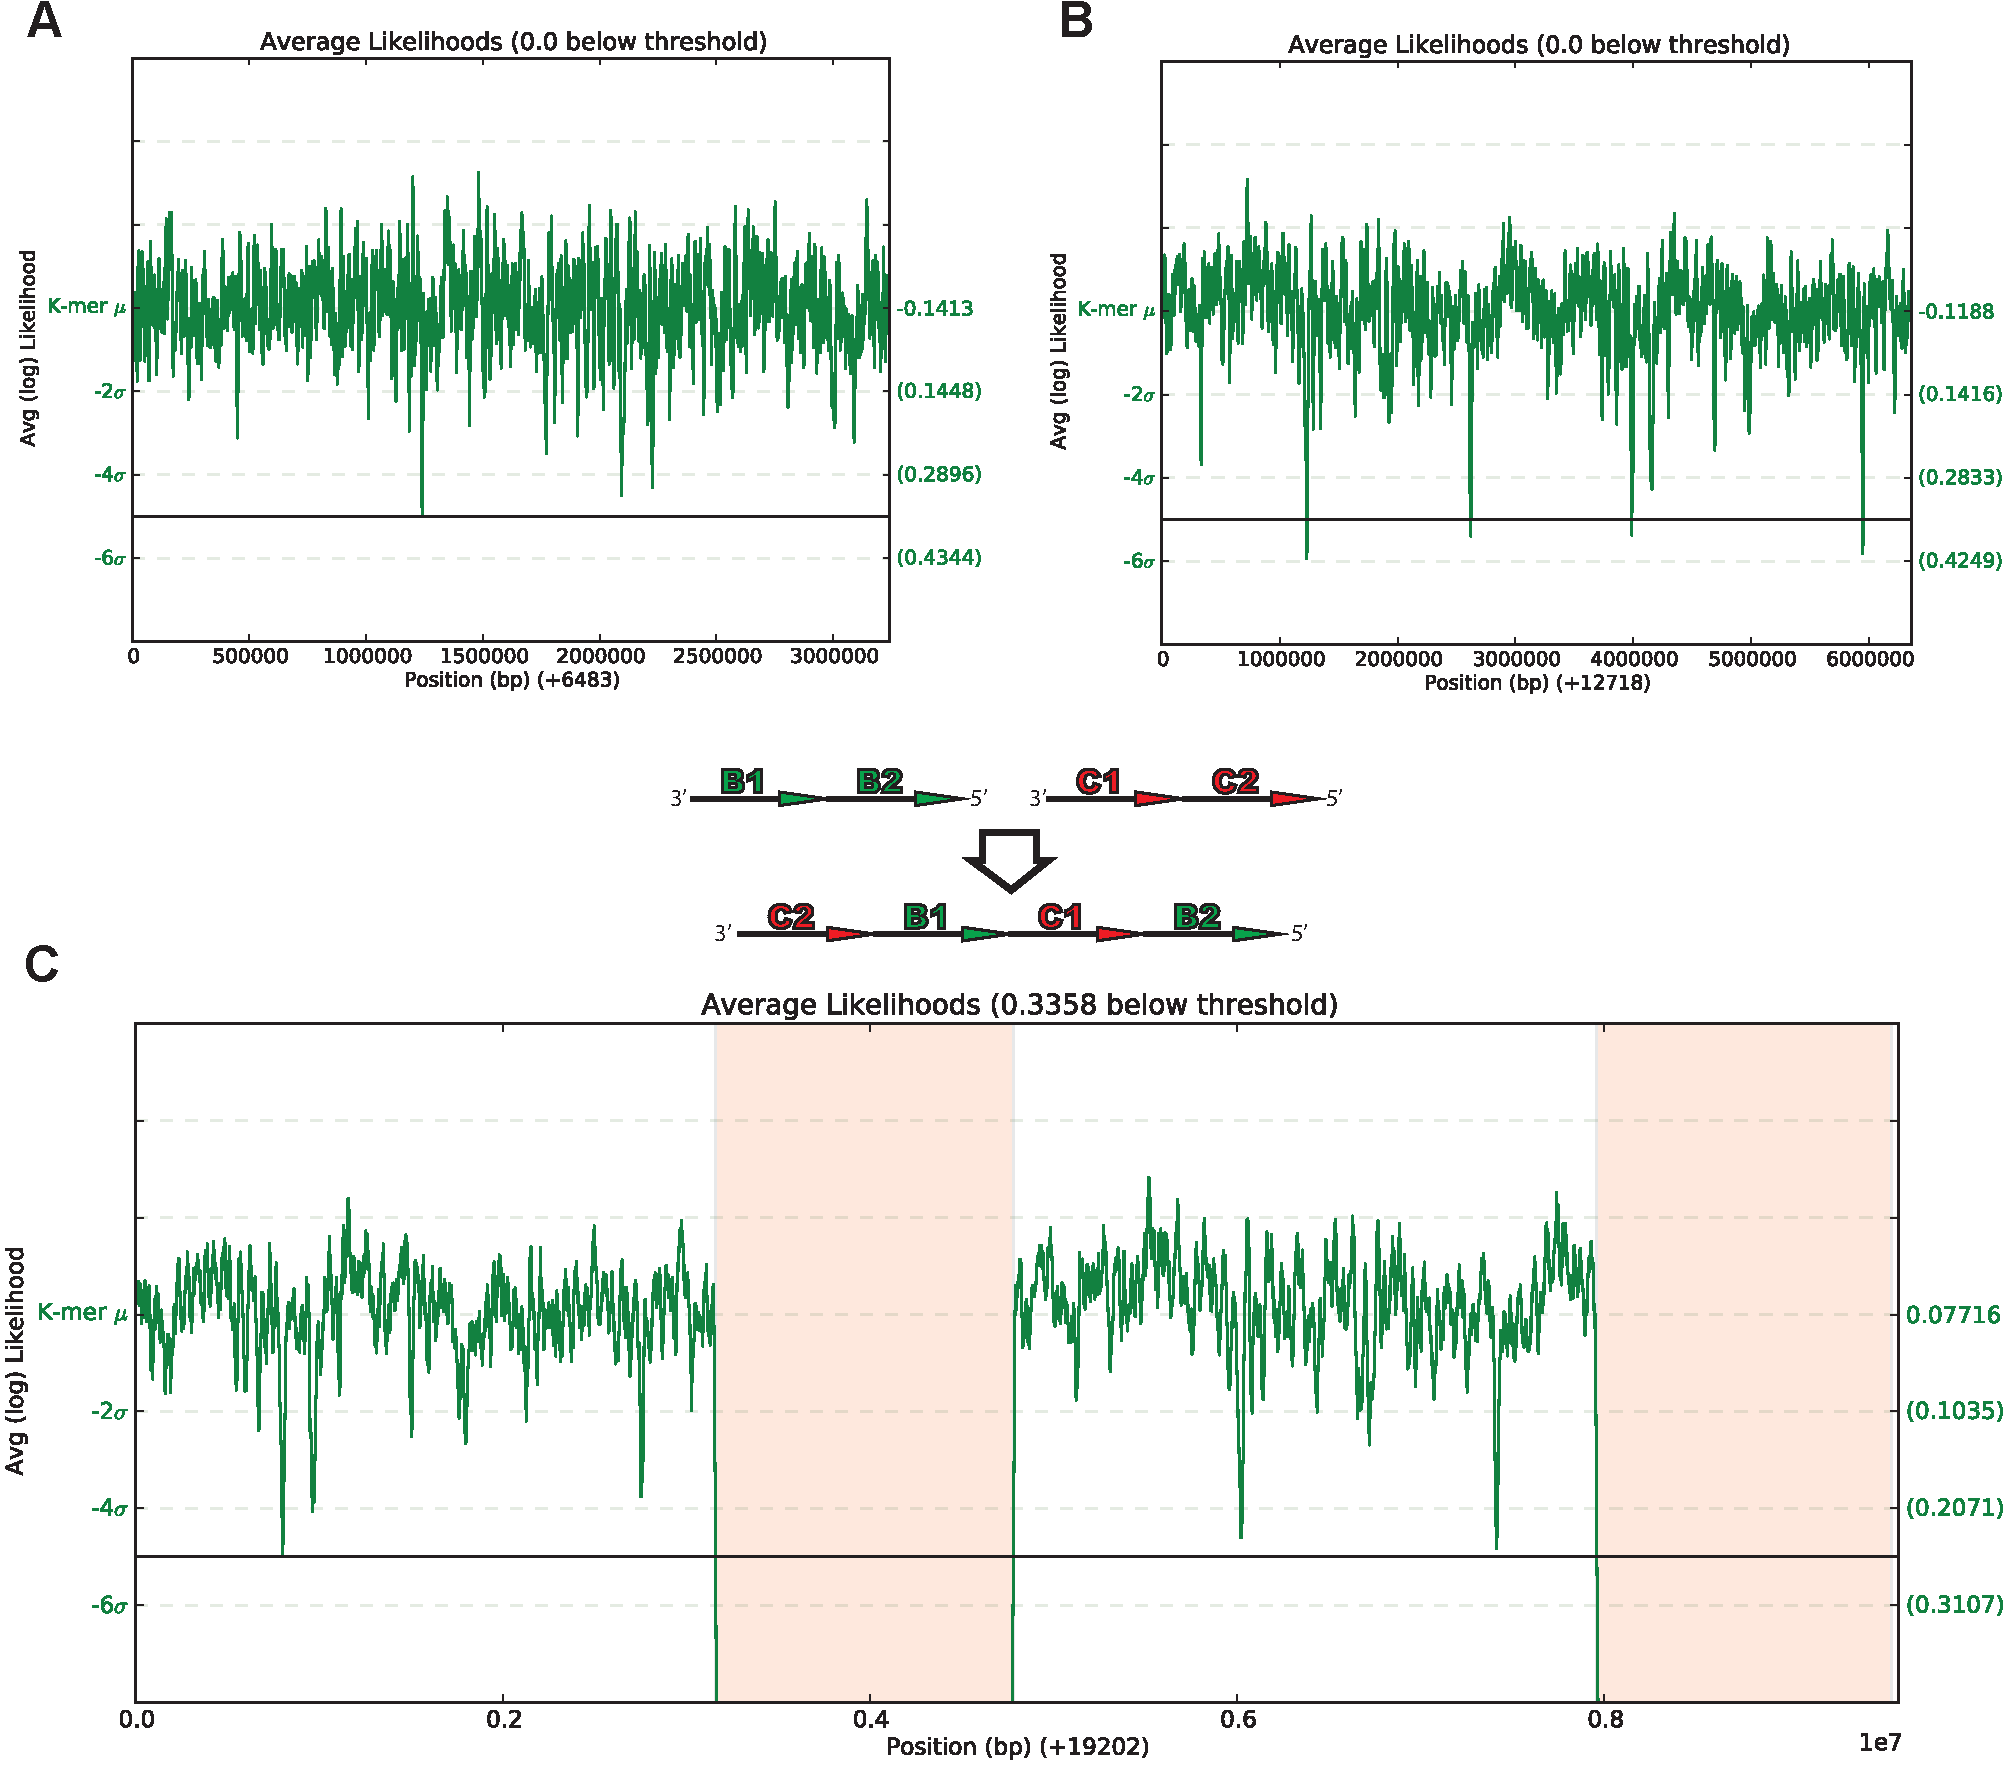
\includegraphics[height = 7cm]{figures/ALE/Clark_Fig4b.pdf}
\end{center}
}

\frame{\frametitle{Discovery of errors in real genome assemblies}
\begin{center}
 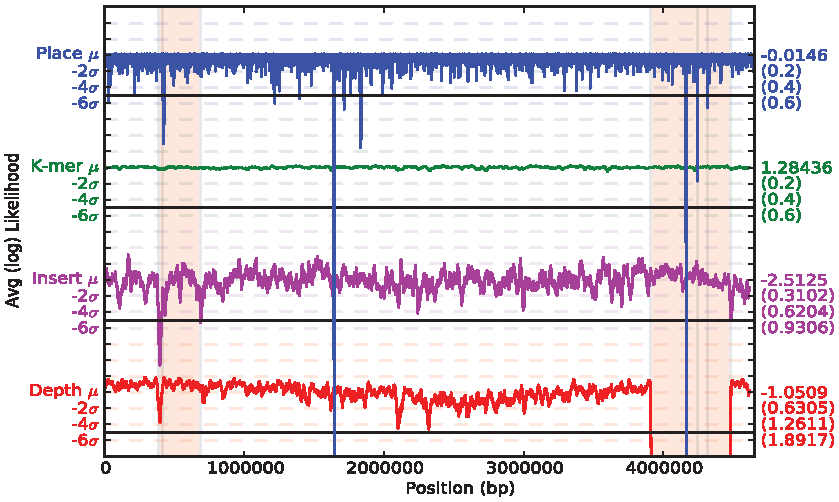
\includegraphics[height = 6cm]{figures/ALE/fig5_top.pdf}
\end{center}
}

\frame{\frametitle{Discovery of errors in real genome assemblies}
\begin{center}
 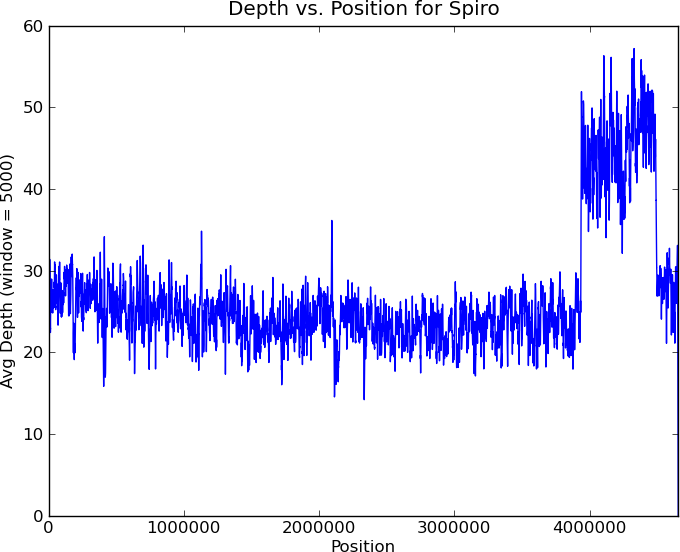
\includegraphics[height = 7cm]{depthVsPosSpiro.png}
\end{center}
}

\frame{\frametitle{Discovery of errors in real genome assemblies}
\begin{center}
 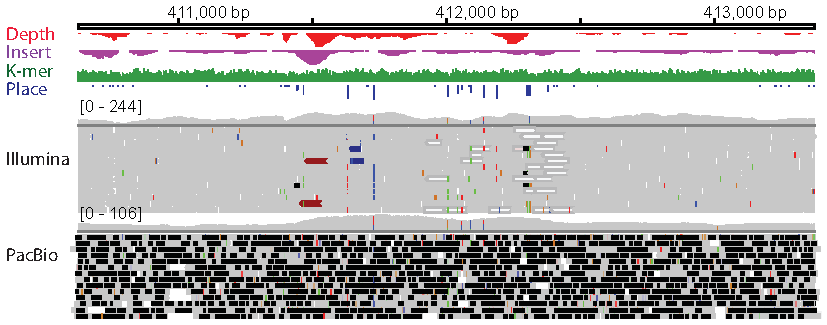
\includegraphics[height = 4cm]{figures/ALE/fig5_mid.pdf}
\end{center}
}

\frame{\frametitle{Discovery of errors in real genome assemblies}
\begin{center}
 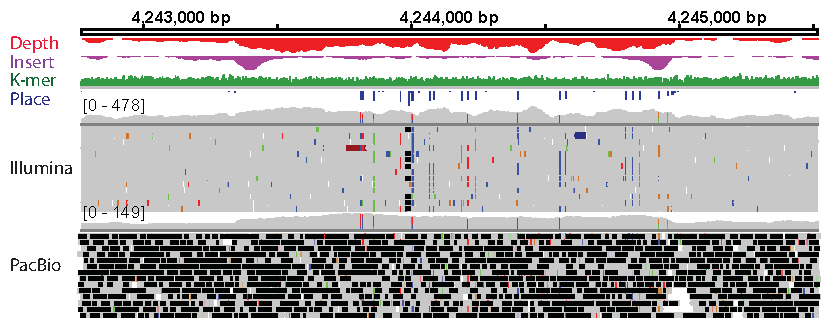
\includegraphics[height = 4cm]{figures/ALE/fig5_bot.pdf}
\end{center}
}

\frame{\frametitle{Performance with Pacific Biosciences RS data}
\begin{center}
    \footnotesize
            \begin{tabular}{cccccc}
Operation & Mutation & Position & 548x& 50x & 548x\\
Type & Details & & Evicon & Rank & Rank\\
 & & & (PacBio) & (ALE) & (ALE)\\
\hline
Sub & C $\rightarrow$ A & 881 & 1 & 5 & 5\\
Ins & CC $\rightarrow$ CCC & 2161 & - & 14 & 12\\
Del & G $\rightarrow$ - & 3681 & 1 & 9 & 8\\
N/A & - & 15712 & - & 7 & -\\
Del & AACGGGCAGA & 16561 & 1 & 4 & 4\\
Ins & AACGGGCAGA & 17030 & 1 & 3 & 2\\
Sub & A $\rightarrow$ G & 22881 & 1 & 10 & 7\\
Sub & T $\rightarrow$ A & 28561 & 1 & 11 & 10\\
Del & T & 34560 & 1 & 12 & 11\\
Sub & G $\rightarrow$ C & 36560 & 1 & 8 & 9\\
Ins & ACGTACGT & 40721 & 1 & 1 & 1\\
N/A & - & 41318 & - & 13 & -\\
Del & TCATCGCG & 43200 & - & 6 & 6\\
Ins & C & 47600 & 1 & 2 & 3
\end{tabular}
\end{center}
}

{
\usebackgroundtemplate{\vspace{2cm}
\includegraphics[width=\paperwidth]{ALE.png}}

\frame{\frametitle{ALE Conclusion}

In ALE we have developed an algorithm and software package that
\begin{itemize}
 \item Can validate assemblies in a rigorous and probabilistic way$^{\star}$
 \item Allows for the quick discovery of errors in assemblies
 \item Can validate metagenomic assemblies and datasets$^{\star}$
 \item Can be used to help ``finish'' genomes
 \item Open source, easy to install, easy to fit into a pipeline
\end{itemize}
}


}

\section{Parallel Optimization}

\subsection{Introduction}
\frame{\frametitle{Expected Parallel Improvement}

\begin{center}
We want a fast/efficient, derivative-free and global optimization algorithm for an expensive to evaluate, ``black box" function $f$.
\[\max_{x \in A} f(x).\]

The function $f$ has domain $A \subseteq \mathbb{R}^{d}$, possibly constrained.

\[\]

This function can be anything, like an assembly likelihood given either the reference or some parameters for an assembler.
\end{center}

}

\frame{\frametitle{The math (figures next!)}
We begin with a Gaussian process prior on a continuous function $f$.

\[f \sim \text{GP}(\mu(\cdot), \Sigma(\cdot, \cdot))\]

\[(f(x_{1}), \ldots, f(x_{n})) \sim N\left( \left[ \begin{tabular}{c} $\mu(x_{1})$ \\ $\vdots$ \\ $\mu(x_{n})$ \end{tabular} \right] , \left[ \begin{tabular}{ccc} $\Sigma(x_{1}, x_{1})$ & $\cdots$ & $\Sigma(x_{n}, x_{1})$ \\ $\vdots$ & $\ddots$ & $\vdots$ \\ $\Sigma(x_{1}, x_{n})$ & $\cdots$ & $\Sigma(x_{n},x_{n}$ \end{tabular} \right] \right)\]

\[\mu_{n}(x_{\star}) = K(\vec{x}_{\star}, \textbf{X} )K(\textbf{X},\textbf{X})^{-1}\vec{y}\]

\[\Sigma_{n}(x_{\star}) = K(\textbf{x$_{\star}$}, \textbf{x$_{\star}$}) - K(\textbf{x$_{\star}$}, \textbf{X}) K(\textbf{X}, \textbf{X})^{-1} K(\textbf{X}, \textbf{x$_{\star}$})\]

\[K(\vec{y}, \vec{z})_{ij} = \text{cov}(y_{i}, z_{j})\]

}

\frame{\frametitle{GPP evolving with information}
\begin{center}
 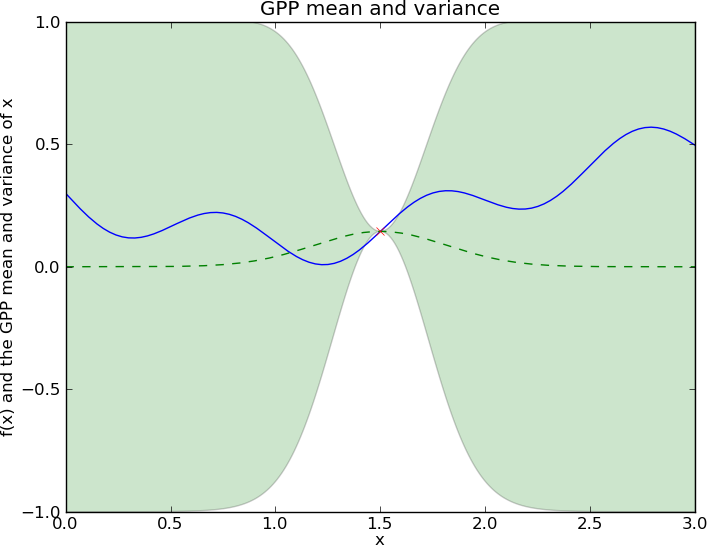
\includegraphics[height = 6.4cm]{EPIgif1.png}
\end{center}
}
\frame{\frametitle{GPP evolving with information}
\begin{center}
 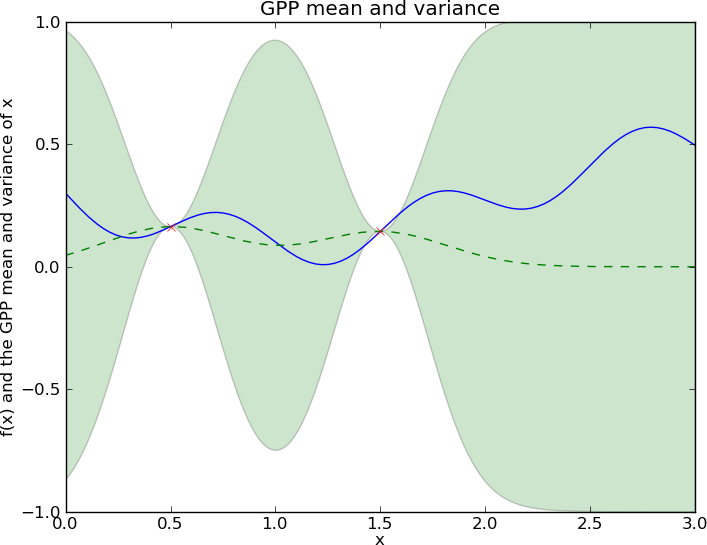
\includegraphics[height = 6.4cm]{EPIgif2.png}
\end{center}
}
\frame{\frametitle{GPP evolving with information}
\begin{center}
 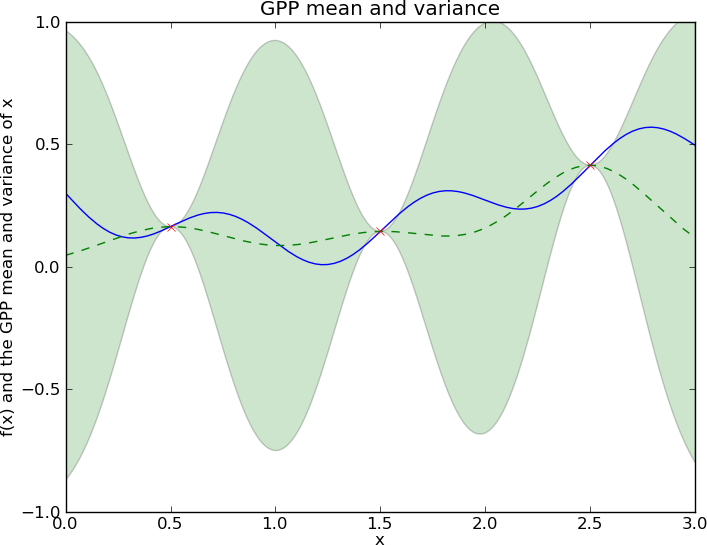
\includegraphics[height = 6.4cm]{EPIgif3.png}
\end{center}
}
\frame{\frametitle{GPP evolving with information}
\begin{center}
 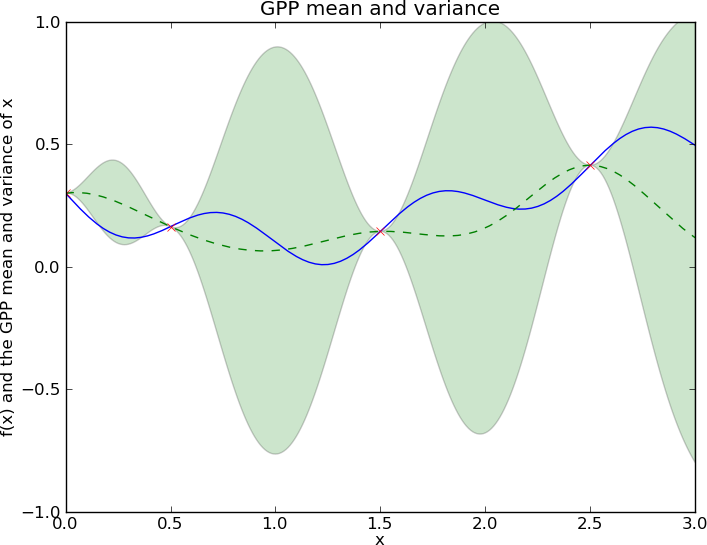
\includegraphics[height = 6.4cm]{EPIgif4.png}
\end{center}
}
\frame{\frametitle{GPP evolving with information}
\begin{center}
 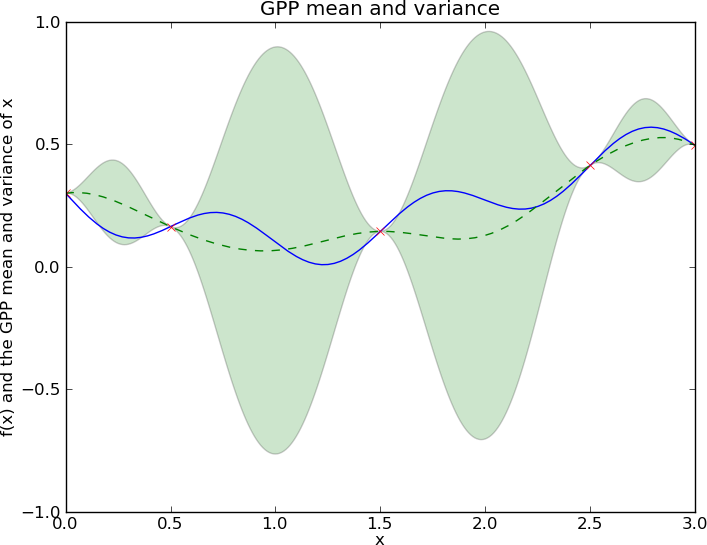
\includegraphics[height = 6.4cm]{EPIgif5.png}
\end{center}
}
\frame{\frametitle{GPP evolving with information}
\begin{center}
 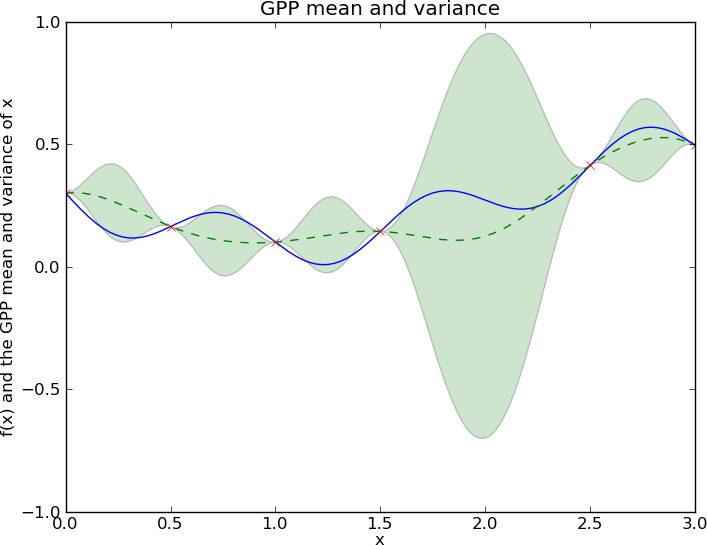
\includegraphics[height = 6.4cm]{EPIgif6.png}
\end{center}
}
\frame{\frametitle{GPP evolving with information}
\begin{center}
 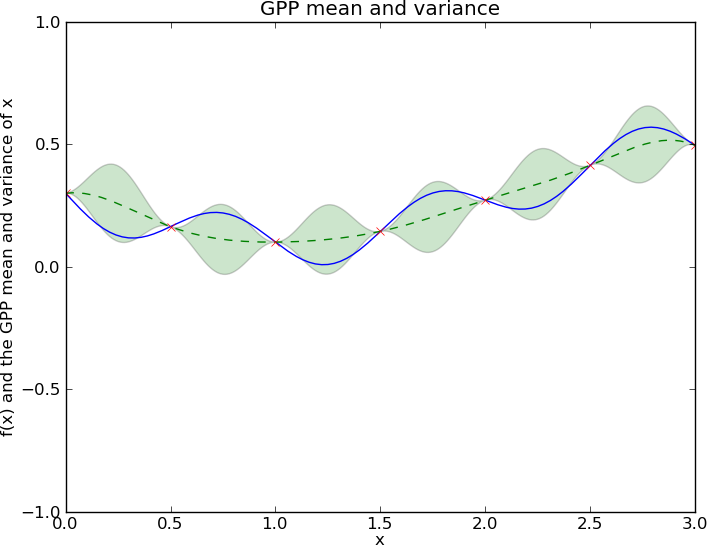
\includegraphics[height = 6.4cm]{EPIgif7.png}
\end{center}
}

\subsection{EI}
\frame{\frametitle{Expected Improvement}

\[\text{EI}(x) = \mathbb{E}_{n} \left[\left[ f(x) - f_{n}^{\star} \right]^{+} \right] = \mathbb{E} \left[ f_{n+1}^{\star} - f_{n}^{\star} | x_{n} = x\right]\]

\begin{center}where $f_{n}^{\star} = \max_{m \leq n} f(x_{m})$.\end{center}

The core of this idea is that we can calculate the expected improvement for simultaneous evaluation of points $x_{n+1}, \ldots, x_{n+l} = \vec{x}$ as
\[\text{EI}(x_{n+1}, \ldots, x_{n+l}) = \mathbb{E}_{n}\left[\left[\max\left\{f(x_{n+1}), \ldots, f(x_{n+l})\right\} - f_{n}^{\star}\right]^{+}\right].\]

The optimization then approximates the solution to

\[\argmax_{\vec{x} \in \mathbb{R}^{d \times l}} \text{EI}(\vec{x}).\]

}

\frame{\frametitle{Expected Improvement 2-D}
\begin{center}
 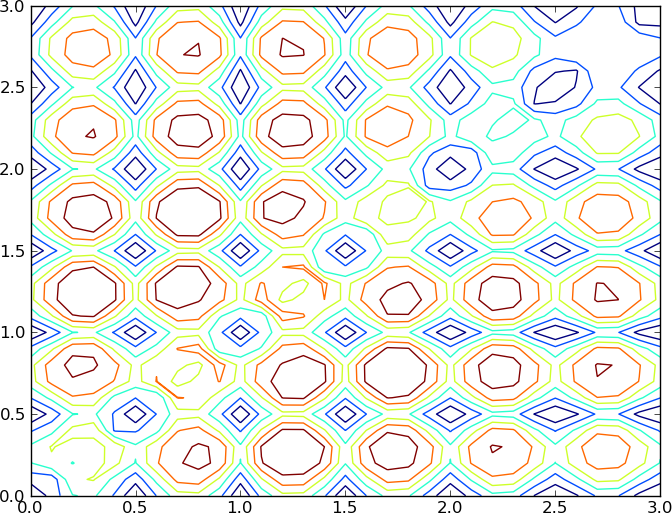
\includegraphics[height = 6.4cm]{peterMeeting020911_p6_analyticT.png}
\end{center}
}

\frame{\frametitle{Expected Improvement 2-D}
To optimize $\text{EI}(\vec{x})$, we calculate stochastic gradients

\[g(\vec{x}) = \bigtriangledown \text{EI}(\vec{x})\]

Which results in (skipping some derivations for the sake of time/sanity)

\[ \frac{\partial}{\partial x_{\star t}} \mu_{\star i} = \left\{ \begin{tabular}{cc}
                                                                  $\sum_{j = 1}^{N} \left(K^{-1} \vec{y} \right)_{j} \frac{\partial}{\partial x_{\star i}} \text{cov}(x_{\star i}, X_{j})$ & for $i = t$ \\
								  0 & otherwise
                                                                 \end{tabular}\right.
\]

\tiny
\[
  \frac{\partial}{\partial x_{\star t}} \Sigma_{ij} = \left\{ \begin{tabular}{cc}
        $2 \sum_{p = 1}^{N} \sum_{q = 1}^{N} K^{-1}_{qp} \left( \mbox{cov}(x_{\star i}, X_{q}) \frac{\partial}{\partial x_{\star i}} \mbox{cov}(x_{\star i}, X_{p}) \right)$ & $t = i = j$ \\
        $\sum_{p = 1}^{N} \sum_{q = 1}^{N} K^{-1}_{qp} \mbox{cov}(x_{\star j}, X_{p}) \frac{\partial}{\partial x_{\star i}} \mbox{cov}(x_{\star i}, X_{q})$ & $t = i \neq j$ \\
							$\sum_{p = 1}^{N} \sum_{q = 1}^{N} K^{-1}_{qp} \mbox{cov}(x_{\star i}, X_{p}) \frac{\partial}{\partial x_{\star j}} \mbox{cov}(x_{\star j}, X_{q})$ & $t = j \neq i$ \\
							$0$ & otherwise
                                                      \end{tabular} \right.
\]

\normalsize

Which we use to inform the algorithm for the differentiation of the Cholesky decomposition... (see code/paper)
}

\frame{\frametitle{Stochastic Gradient of the Expected Improvement using MC}
\begin{center}
 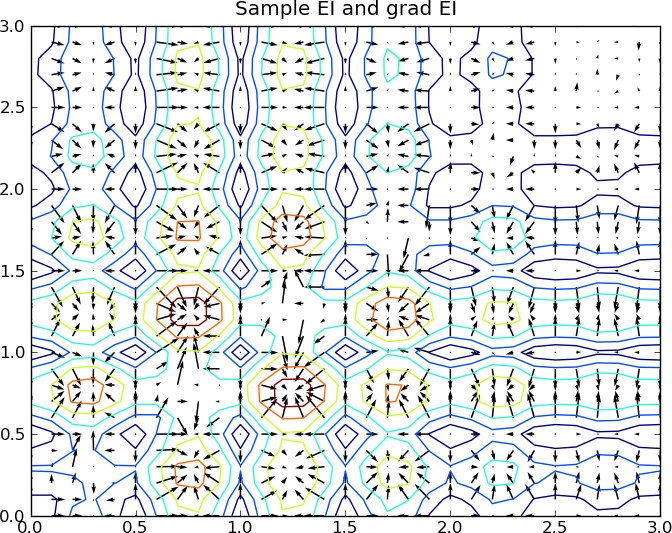
\includegraphics[height = 6.4cm]{041911_sampEIandGradEI.png}
\end{center}
}

\subsection{EPI algorithm}
\frame{\frametitle{The Algorithm}

The Algorithm
\begin{enumerate}
 \item Choose the set of points with the highest EI
 \item As nodes return values search for new best EI along the space constrained by running simulations
\end{enumerate}

\[\vec{x}_{i}^{(t+1)} = \vec{x}_{i}^{(t)} + \frac{a}{t^{\gamma}} \nabla_{\vec{x}_{i}} {\rm EI}\left(\vec{P}^{(t)} | \vec{X}\right)\]
\[\left|\vec{x}_{i}^{(t+1)} - \vec{x}_{i}^{(t)}\right| < \epsilon\]
}

\frame{\frametitle{Multistart paths (1/5)}
\begin{center}
 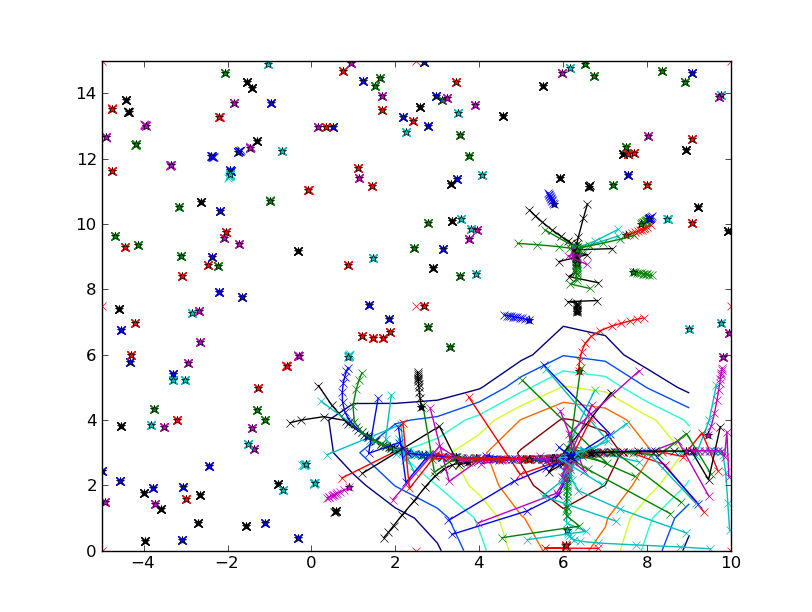
\includegraphics[height = 7cm]{figures/EPI/branin_pk_256singles_EI_max_1.png}
\end{center}
}

\frame{\frametitle{Multistart paths (2/5)}
\begin{center}
 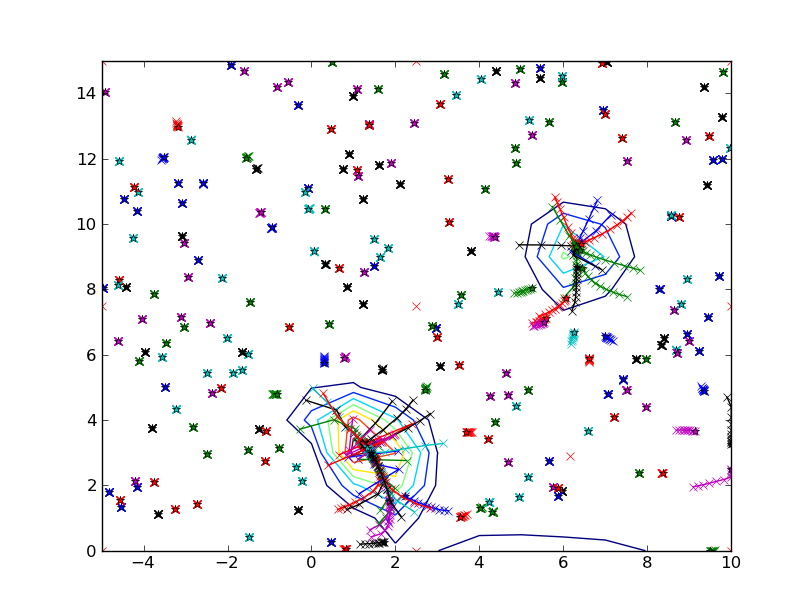
\includegraphics[height = 7cm]{figures/EPI/branin_pk_256singles_EI_max_2.png}
\end{center}
}

\frame{\frametitle{Multistart paths (3/5)}
\begin{center}
 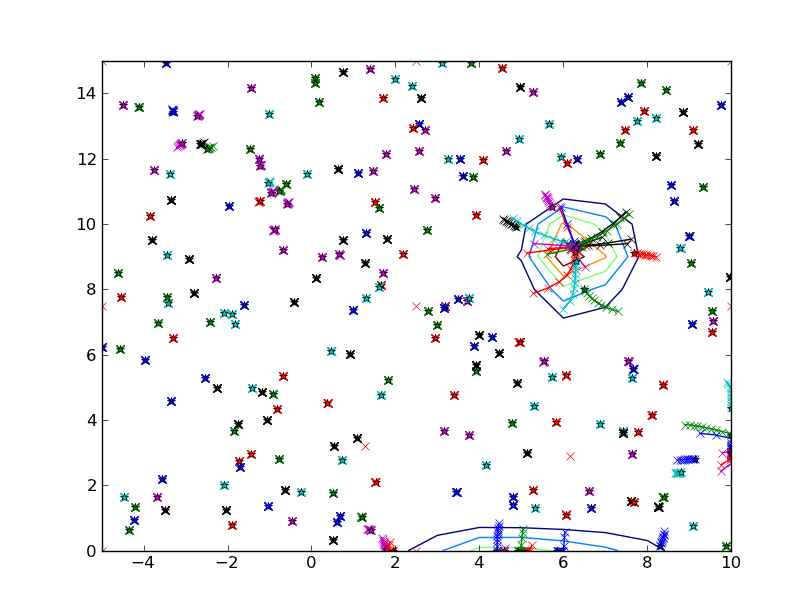
\includegraphics[height = 7cm]{figures/EPI/branin_pk_256singles_EI_max_3.png}
\end{center}
}

\frame{\frametitle{Multistart paths (4/5)}
\begin{center}
 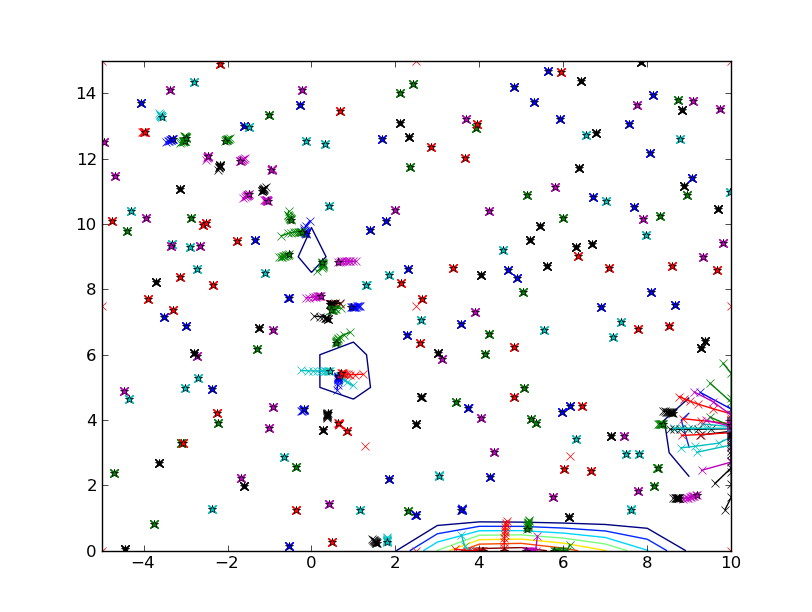
\includegraphics[height = 7cm]{figures/EPI/branin_pk_256singles_EI_max_4.png}
\end{center}
}

\frame{\frametitle{Multistart paths (5/5)}
\begin{center}
 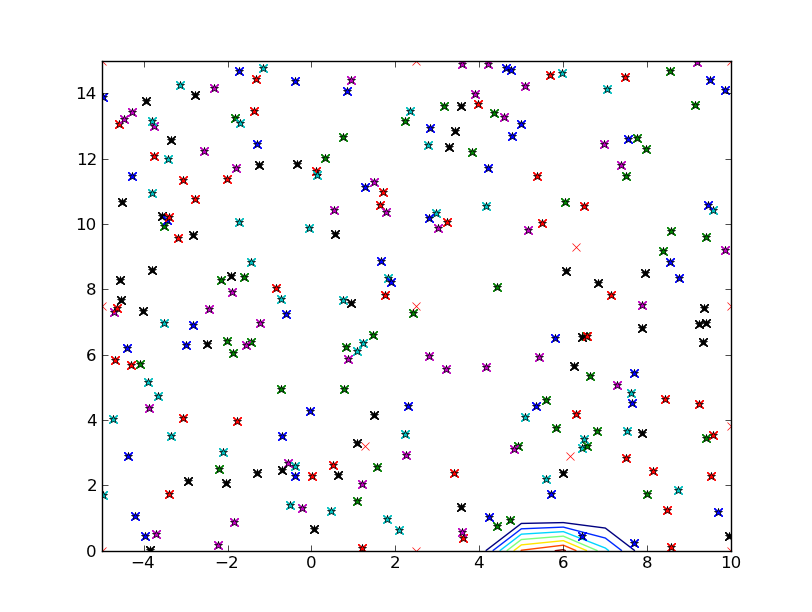
\includegraphics[height = 7cm]{figures/EPI/branin_pk_256singles_EI_max_5.png}
\end{center}
}

\frame{\frametitle{Speedup}
\begin{center}
 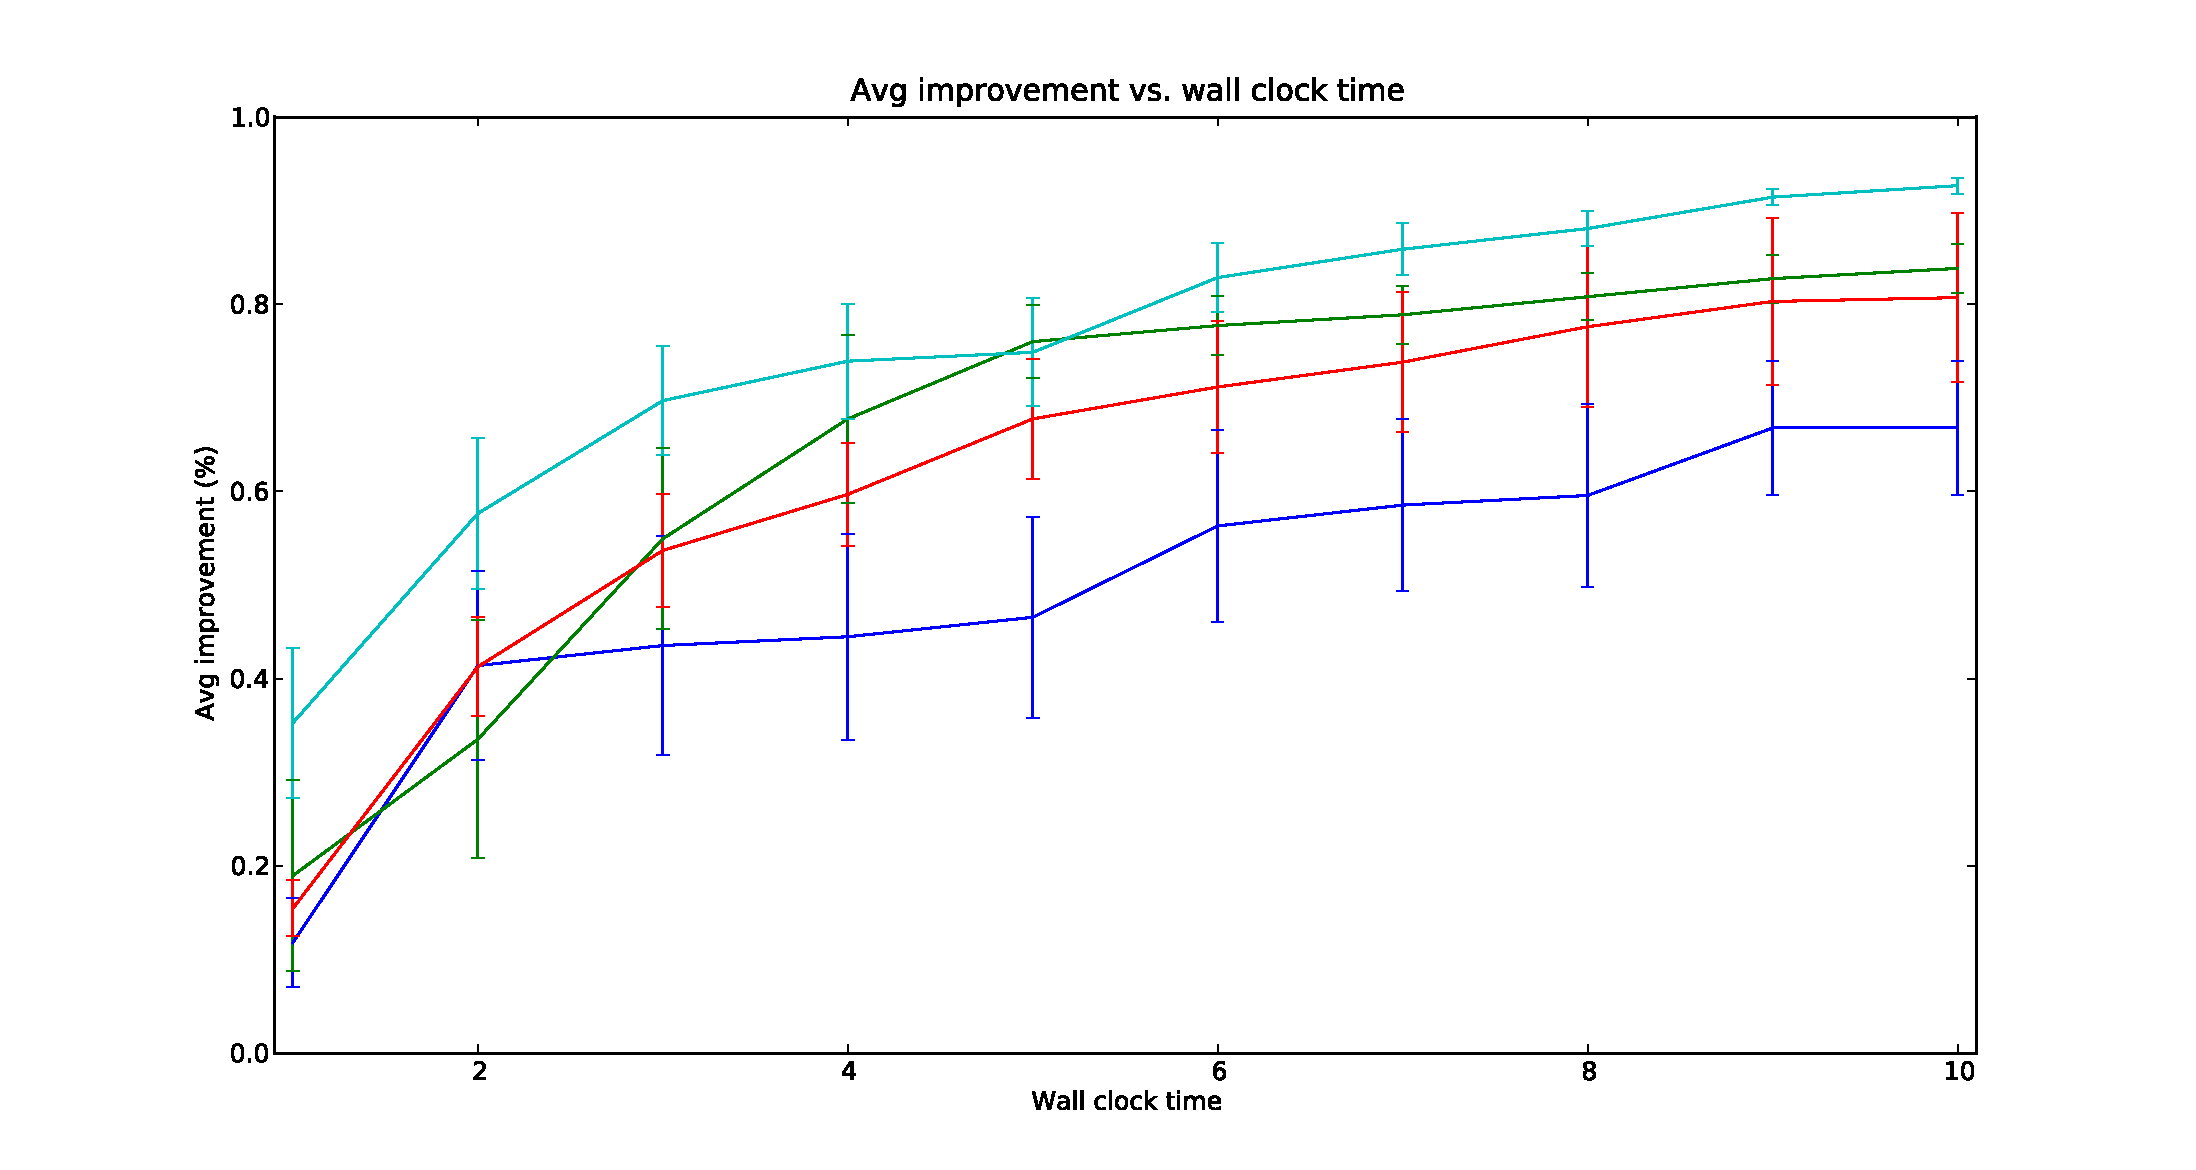
\includegraphics[height = 6.4cm]{figures/EPI/speedup_vs_wallclock_8_core_9_its.pdf}
\end{center}
}

\frame{\frametitle{EPI Conclusion}

WHAT WE DID
}

{
\usebackgroundtemplate{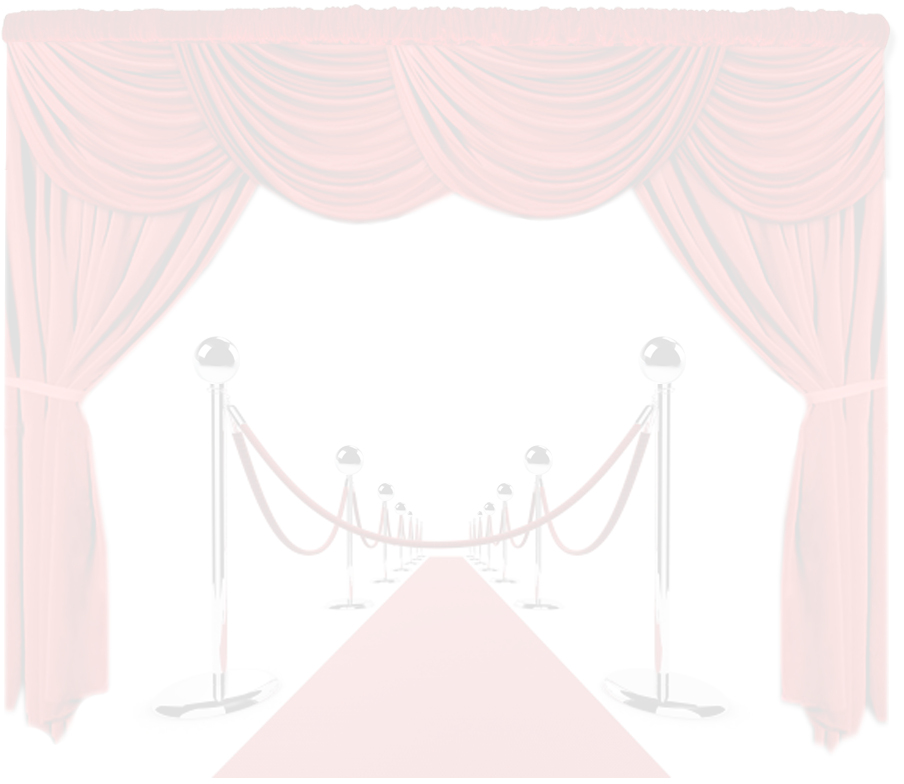
\includegraphics[width=\paperwidth]{VRbackground.jpg}}

\frame{\frametitle{Velvetrope (Part III of thesis)}

Developed an algorithm and software package that

\begin{itemize}
 \item Finds motifs in sequences using a novel statistical model
 \item Is faster than the current methods (GPU implementation, CUDA)
 \item Can handle cases other methods cannot
 \item Natively allows for quick analysis of aggregate data
 \item Is open source and easy to fit into a pipeline
\end{itemize}
}

}

\frame{
\frametitle{Project status}

\begin{tabular}{c|rl}
    \hline 
     & Software: & github.com/sc932/ALE \\
     & & (UoI/CNSA open source license) \\
     ALE & Presented: & SC11, SIAM CSE11, DOE CSGF11 \\
      & & INFORMS10, JGI Seminar \\
      & Paper: & submitted to Bioinformatics \\
      \hline
     & Software: & github.com/sc932/EPI \\
     EPI & & (UoI/CNSA open source license) \\
      & Presented: & SC12, DOE CSGF12 \\
      & Paper: & in preperation \\
\hline
     & Software: & github.com/sc932/Velvetrope \\
     & & (GPL v2 open source license) \\
     Velvetrope & Presented: & SC10, DOE CSGF10 \\
      & Paper: & profiled in DIEXIS \\
\hline
\end{tabular}

}

\frame{
\frametitle{Acknowledgements}


\includegraphics[height = 1.5cm]{csgf.png}$\hspace*{.3cm}$
\includegraphics[height = 1.5cm]{JGI.jpg}$\hspace*{.3cm}$
\includegraphics[height = 1.5cm]{LANL.png}$\hspace*{.3cm}$
\includegraphics[height = 1.5cm]{Cornell.jpg}

\begin{itemize}
 \item DOE Computational Science Graduate Fellowship
 \item Advisor: Peter Frazier (Cornell ORIE)
 \item DOE Joint Genome Institute (JGI) Genome Analysis Group
 \begin{itemize}
  \item Zhong Wang (Mentor)
  \item Rob Egan (Co-Mentor)
 \end{itemize}
 \item Los Alamos National Laboratory (LANL) Metagenomics Group
 \begin{itemize}
  \item Nick Hengartner (Mentor)
  \item Joel Berendzen (Co-Mentor)
 \end{itemize}
 \item Committee \ \ \ \ \ \ \ \ \ \ \ \ \ \ \ \ \ \ \ \ \ \ \ \ \ \ \ \ \ \ \ \ \ \ \ \ DOE Grants
 \begin{itemize}
  \item Steve Strogatz (Math) \ \ \ \ \ \ \ \ \ \ \ \ \ \ \ \ \ \ \ DE-FG02-97ER25308
  \item Bart Selman (CS) \ \ \ \ \ \ \ \ \ \ \ \ \ \ \ \ \ \ \ \ \ \ \ \ \ DE-AC02-05CH11231
  \item Jim Renegar (Math proxy)
 \end{itemize}

\end{itemize}

\begin{picture}(0.1,0.1)
     \put(260,50){
\includegraphics[height = 1cm]{nersc.jpg}}
  \end{picture}


}

\end{document}
